\documentclass[12pt]{article}\usepackage[]{graphicx}\usepackage[]{xcolor}
% maxwidth is the original width if it is less than linewidth
% otherwise use linewidth (to make sure the graphics do not exceed the margin)
\makeatletter
\def\maxwidth{ %
  \ifdim\Gin@nat@width>\linewidth
    \linewidth
  \else
    \Gin@nat@width
  \fi
}
\makeatother

\definecolor{fgcolor}{rgb}{0.345, 0.345, 0.345}
\newcommand{\hlnum}[1]{\textcolor[rgb]{0.686,0.059,0.569}{#1}}%
\newcommand{\hlstr}[1]{\textcolor[rgb]{0.192,0.494,0.8}{#1}}%
\newcommand{\hlcom}[1]{\textcolor[rgb]{0.678,0.584,0.686}{\textit{#1}}}%
\newcommand{\hlopt}[1]{\textcolor[rgb]{0,0,0}{#1}}%
\newcommand{\hlstd}[1]{\textcolor[rgb]{0.345,0.345,0.345}{#1}}%
\newcommand{\hlkwa}[1]{\textcolor[rgb]{0.161,0.373,0.58}{\textbf{#1}}}%
\newcommand{\hlkwb}[1]{\textcolor[rgb]{0.69,0.353,0.396}{#1}}%
\newcommand{\hlkwc}[1]{\textcolor[rgb]{0.333,0.667,0.333}{#1}}%
\newcommand{\hlkwd}[1]{\textcolor[rgb]{0.737,0.353,0.396}{\textbf{#1}}}%
\let\hlipl\hlkwb

\usepackage{framed}
\makeatletter
\newenvironment{kframe}{%
 \def\at@end@of@kframe{}%
 \ifinner\ifhmode%
  \def\at@end@of@kframe{\end{minipage}}%
  \begin{minipage}{\columnwidth}%
 \fi\fi%
 \def\FrameCommand##1{\hskip\@totalleftmargin \hskip-\fboxsep
 \colorbox{shadecolor}{##1}\hskip-\fboxsep
     % There is no \\@totalrightmargin, so:
     \hskip-\linewidth \hskip-\@totalleftmargin \hskip\columnwidth}%
 \MakeFramed {\advance\hsize-\width
   \@totalleftmargin\z@ \linewidth\hsize
   \@setminipage}}%
 {\par\unskip\endMakeFramed%
 \at@end@of@kframe}
\makeatother

\definecolor{shadecolor}{rgb}{.97, .97, .97}
\definecolor{messagecolor}{rgb}{0, 0, 0}
\definecolor{warningcolor}{rgb}{1, 0, 1}
\definecolor{errorcolor}{rgb}{1, 0, 0}
\newenvironment{knitrout}{}{} % an empty environment to be redefined in TeX

\usepackage{alltt}
\usepackage[spanish,es-nodecimaldot]{babel}%*** idioma ***
\usepackage[utf8]{inputenc}
\usepackage{multirow,array,graphicx}
\usepackage{fancyhdr}
\usepackage{geometry}%**geometria
\usepackage[table]{xcolor}

\geometry{
	left = 10 mm, right = 20 mm, top = 50mm, bottom = 30mm, headheight = 40mm }

\pagestyle{fancy}
\fancyhf{}
\usepackage[useregional]{datetime2}%**fecha		
\usepackage{graphicx} %para cargar figuras
\usepackage{soul}
\usepackage{float}
\usepackage{xcolor, colortbl}
\usepackage{pdfpages}
%para hacer lista con sub niveles
\usepackage{enumitem}
%para configurar tamaño de la letra en una tabla
\usepackage{adjustbox}

%para notas y fuentes de tablas
\usepackage{caption}
%definiendo el color
\definecolor{color}{rgb}{0.37, 0.62, 0.63}
%para diferenciar la ultima pagina
\usepackage{lastpage}
\usepackage{longtable}
\newcommand{\num}{009}
\newcommand{\gerente}{Ing Maria Teresa Paucar Ordoñez}
\newcommand{\cargog}{COORDINADORA DEL PROYECTO}
\newcommand{\remitente}{Econ Percy Alberth Hinojosa Cahuana}
\newcommand{\asunto}{Remito informe de actividades realizadas hasta la fecha}
\newcommand{\referencia}{Contrato de trabajo modalidad servici especifico N 737-2023-IMA-DE}
\newcommand{\dia}{11}
\newcommand{\mes}{marzo}
\newcommand{\anio}{2024}
\newcommand{\distrito}{Livitaca}
\newcommand{\comunidad}{Chilloroya}
\newcommand{\nombrepi}{RECUPERACION DEL SERVICIO ECOSISTEMICO DE REGULACION HIDRICA EN LA CUENCA ALTA DEL RIO APURIMAC, DISTRITOS DE COLQUEMARCA, CHAMACA VELILLE, LIVITACA, COPORAQUE, OCORURO, CONDOROMA Y PICHIGUA PROVINCIA DE CHUMBIVILCAS Y ESPINAR, REGIÓN CUSCO}
\newcommand{\icui}{261643}

%%%%CADENA FUNCIONAL
\newcommand{\funcion}{17 AMBIENTE}
\newcommand{\divfuncional}{054 DESARROLLO ESTRATÉGICO, CONSERVACIÓN Y APROVECHAMIENTO SOSTENIBLE DEL PATRIMONIO NATURAL}
\newcommand{\grufuncional}{0120 GESTION INTEGRADA Y SOSTENIBLE DE LOS ECOSISTEMAS}
\newcommand{\secresponsable}{41 AMBIENTAL}
\newcommand{\tipologia}{332 ECOSISTEMAS}
\newcommand{\brecha}{Porcentaje de superficie de ecosistemas degradados que brindan servicios ecosistemicos que requieren de recuperacion}
%% para un mejor orden en los multirow
%\renewcommand{\multirowsetup}{\centering}
%\newlength{\LL}\settowidth{\LL}{texto}

\fancyhead[c]{
	
	\begin{tabular}{|m{1.2cm}|m{2.3cm}|m{2.5cm}|m{1.3cm}|m{3.9cm}|m{5.9cm}|}
		\hline
		\includegraphics[height=2cm,width=1.2cm]{H:/Gore Cusco/img/peru}&\includegraphics[height=1.9cm,width=2.3cm]{H:/Gore Cusco/img/gore}&\cellcolor[rgb]{0.7,0.11,0.11}\textcolor{white}{\textbf{{\small Gobierno Regional de Cusco}}}&\includegraphics[height=1.9cm,width=1.3cm]{H:/Gore Cusco/img/ima}&\cellcolor{gray!100}\textcolor{white}{\textbf{{\small Instituto de Manejo del Agua y Medio Ambiente - IMA}}}&\cellcolor{gray!30}\textbf{{\small Dirección de proyectos Ambientales y Gestión del Conocimiento}}\\
		\hline
		\multicolumn{6}{c}{}\\
		\multicolumn{6}{c}{\textit{"Año del Bicentenario, de la consolidación de nuestra Independencia, y de la conmemoración}}\\
		\multicolumn{6}{c}{\textit{ de las heroicas batallas de Junín y Ayacucho"}}\\
	\end{tabular}
}
%\fancyfoot[C]{\thepage}
\fancyfoot[L]{\includegraphics[scale=0.4]{H:/Gore Cusco/img/firma}}
%para la ultima pagina
\fancypagestyle{lastpage}{
	\fancyhf{}
	\fancyhead[c]{
		
		\begin{tabular}{|m{1.2cm}|m{2.3cm}|m{2.5cm}|m{1.3cm}|m{3.9cm}|m{5.9cm}|}
			\hline
			\includegraphics[height=2cm,width=1.2cm]{H:/Gore Cusco/img/peru}&\includegraphics[height=1.9cm,width=2.3cm]{H:/Gore Cusco/img/gore}&\cellcolor[rgb]{0.7,0.11,0.11}\textcolor{white}{\textbf{{\small Gobierno Regional de Cusco}}}&\includegraphics[height=1.9cm,width=1.3cm]{H:/Gore Cusco/img/ima}&\cellcolor{gray!100}\textcolor{white}{\textbf{{\small Instituto de Manejo del Agua y Medio Ambiente - IMA}}}&\cellcolor{gray!30}\textbf{{\small Dirección de proyectos Ambientales y Gestión del Conocimiento}}\\
			\hline
			\multicolumn{6}{c}{}\\
			\multicolumn{6}{c}{\textit{"Año de la unidad, la paz y el desarrollo"}}
		\end{tabular}
	}
	%\fancyfoot[C]{\thepage}
}
\renewcommand{\headrulewidth}{1pt}


\newenvironment{anexos}[1]
{\begin{titlepage}
		\vspace{10cm}
		\begin{center}{\Huge \textbf{#1}}\end{center}}
	{\end{titlepage}}
\IfFileExists{upquote.sty}{\usepackage{upquote}}{}
\begin{document}
\begin{titlepage}
	\centering
	{\includegraphics[width=0.3\textwidth]{H:/Gore Cusco/img/ima}\par}
	\vspace{1cm}
	{\bfseries\LARGE INSTITUTO DE MANEJO DE AGUA Y MEDIO AMBIENTE \par}
	\vspace{1cm}
	{\scshape\Large Dirección de Proyectos Ambientales y Gestión del Conocimiento \par}
	\vspace{1cm}
	{\scshape\Large Analisis de la encuesta realizada en la comunidad de \comunidad\- del proyecto: \par}
	\vspace{1cm}
	{\itshape\normalsize \textbf{\nombrepi} \par}
	\vfill
	{\Large Autor: \par}
	{\Large \remitente \par}
	\vfill
	{\Large \mes \- \anio \par}
\end{titlepage}
\tableofcontents
\newpage
\listoftables
\newpage
\listoffigures
\newpage
	La encuesta se realizo en la comunidad campesina de \comunidad\- del distrito de distrito, provincia de provincia departamento del Cusco.\\
	\\
	Para esto se considero informacion general de la poblacion, tomando en cuenta el genero, la edad y el recurso que utilizan, en este caso si usan qocha.\\
	\\
	Del genero de las personas encuestadas se puede mostrar lo siguiente:
	\begin{figure}[H]
	\centering
\begin{knitrout}
\definecolor{shadecolor}{rgb}{0.969, 0.969, 0.969}\color{fgcolor}
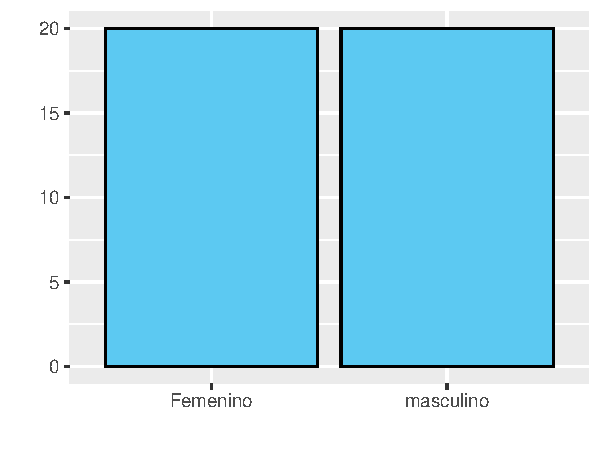
\includegraphics[width=\maxwidth]{figure/uno-1} 
\end{knitrout}
	\caption{Sexo de los encuestados de \comunidad}
	\end{figure}
	Se observa que las cantidades son casi similares, de la cual se observa que los de genero masculino es mayor.
	\section{Datos generales}
	Edad de los encuestados, de la encuesta realizada se tiene la edad de los participantes, como se muestra a continuacion:
	\begin{figure}[H]
	\centering
\begin{knitrout}
\definecolor{shadecolor}{rgb}{0.969, 0.969, 0.969}\color{fgcolor}
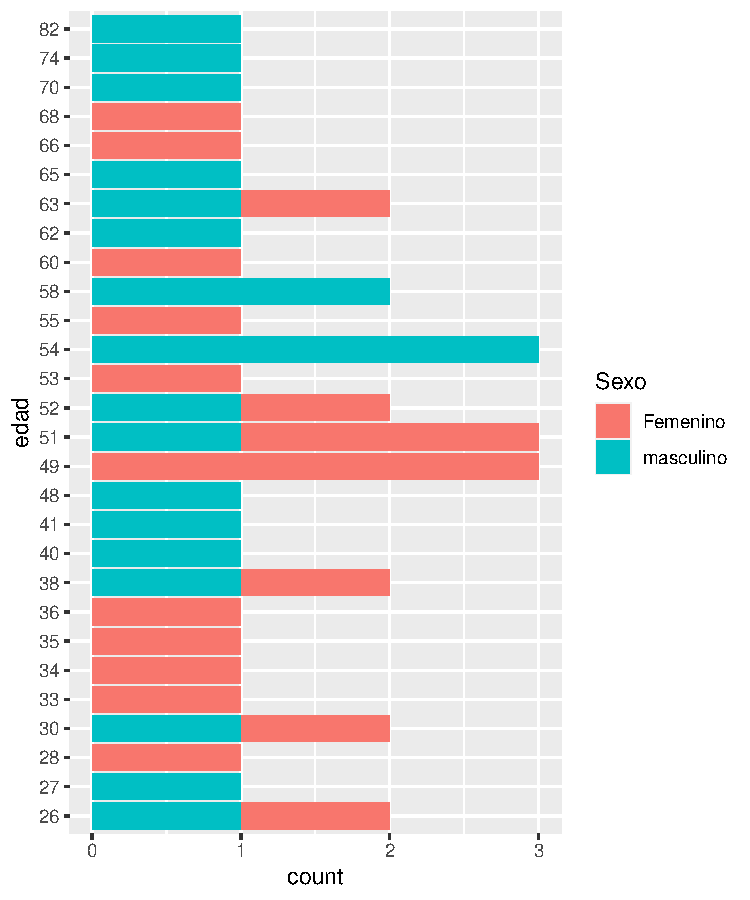
\includegraphics[width=\maxwidth]{figure/dos-1} 
\end{knitrout}
             	
	\caption{Edad de los encuestados de \comunidad}
	\end{figure}
	
	
	
	Se puede observar que el rango de edades va desde 31 hasta 75, siendo la edad de mayor frecuencia la de 42
	\section{Informacion sobre la vivienda}
Se pregunto respecto a la tenencia de la propiedad en la que habitan los encuestados, de la cual se oberva que el 100\% es propia, como se puede observar en la grafica:
	\begin{figure}[H]
	\centering
\begin{knitrout}
\definecolor{shadecolor}{rgb}{0.969, 0.969, 0.969}\color{fgcolor}
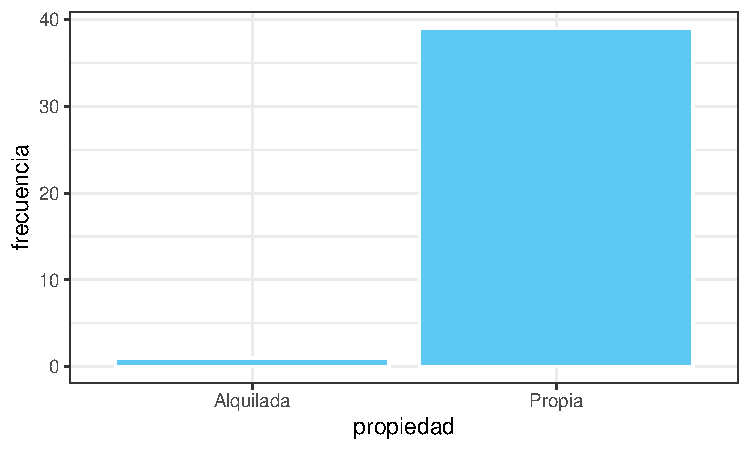
\includegraphics[width=\maxwidth]{figure/tres-1} 
\end{knitrout}
	\caption{Tenencia de la propiedad de los pobladores de \comunidad}
	\end{figure}
	
	Se consulto el tiempo, años, que viven los pobladores en la comunidad, de lo cual se tiene como resultado lo siguiente:
	\begin{figure}[H]
	\centering
\begin{knitrout}
\definecolor{shadecolor}{rgb}{0.969, 0.969, 0.969}\color{fgcolor}
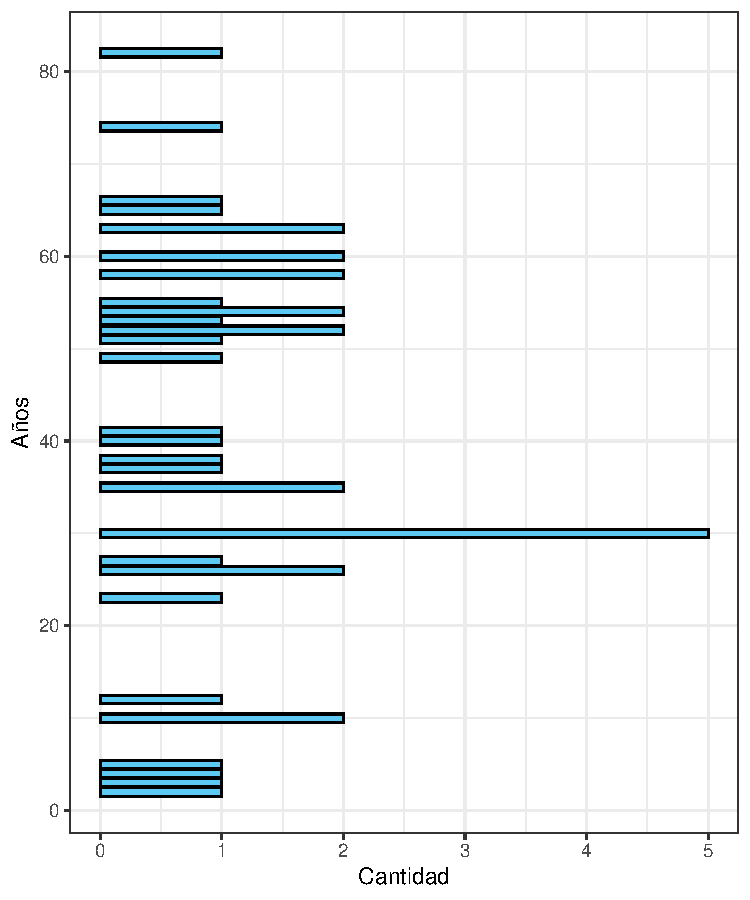
\includegraphics[width=\maxwidth]{figure/cuatro-1} 
\end{knitrout}
	\caption{Años de permanencia de los pobladores en \comunidad}
	\end{figure}
	Se observo que los años que habitan los pobladores van desde 2 a 73, los años que tienen mas frecuencia son de 50 y 20.
	
	Del idioma que los encuestados se identifico que que la mayoria habla español y quechua, como se grafica:
	\begin{figure}[H]
	\centering
\begin{knitrout}
\definecolor{shadecolor}{rgb}{0.969, 0.969, 0.969}\color{fgcolor}
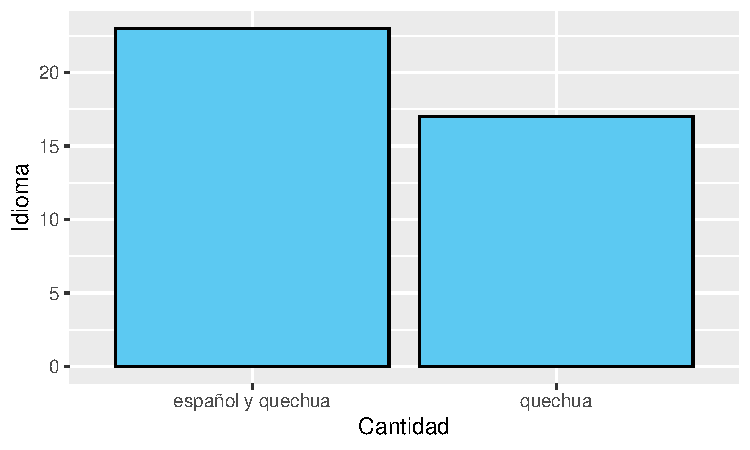
\includegraphics[width=\maxwidth]{figure/cinco-1} 
\end{knitrout}
	\caption{Idioma que habla el poblador}
	\end{figure}
	Se observa que la gran mayoria de los encuestados hablan español y quechua, mientras que solo una pequeña parte habla solo quechua.
	\section{Informacion de servicios}
	De la fuente de agua que los pobladores se abastecen se identifico lo siguiente:
	\begin{figure}[H]
	\centering
\begin{knitrout}
\definecolor{shadecolor}{rgb}{0.969, 0.969, 0.969}\color{fgcolor}
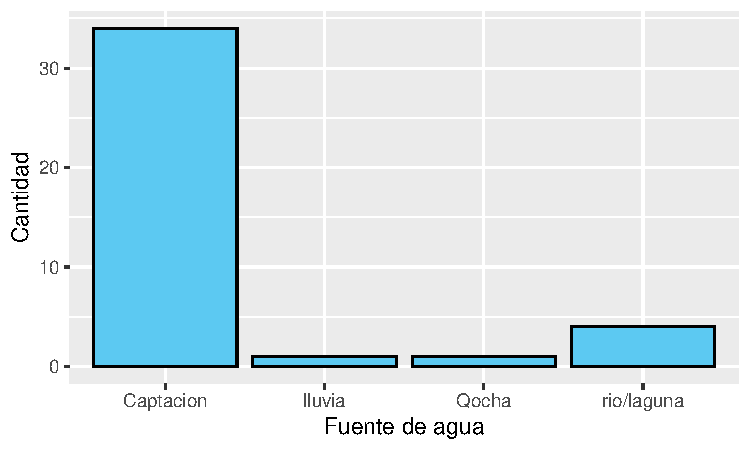
\includegraphics[width=\maxwidth]{figure/seis-1} 
\end{knitrout}
	\caption{Fuente de agua para consumo de agua de los pobladores de \comunidad}
	\end{figure}
	La fuente de manantial y rio/laguna son las que proveen de agua para los pobladores, siendo la de menos uso ojo de agua\\
	\\
	La eliminacion de basura en las viviendas de los pobladores es la siguiente
	\begin{figure}[H]
	\centering
\begin{knitrout}
\definecolor{shadecolor}{rgb}{0.969, 0.969, 0.969}\color{fgcolor}
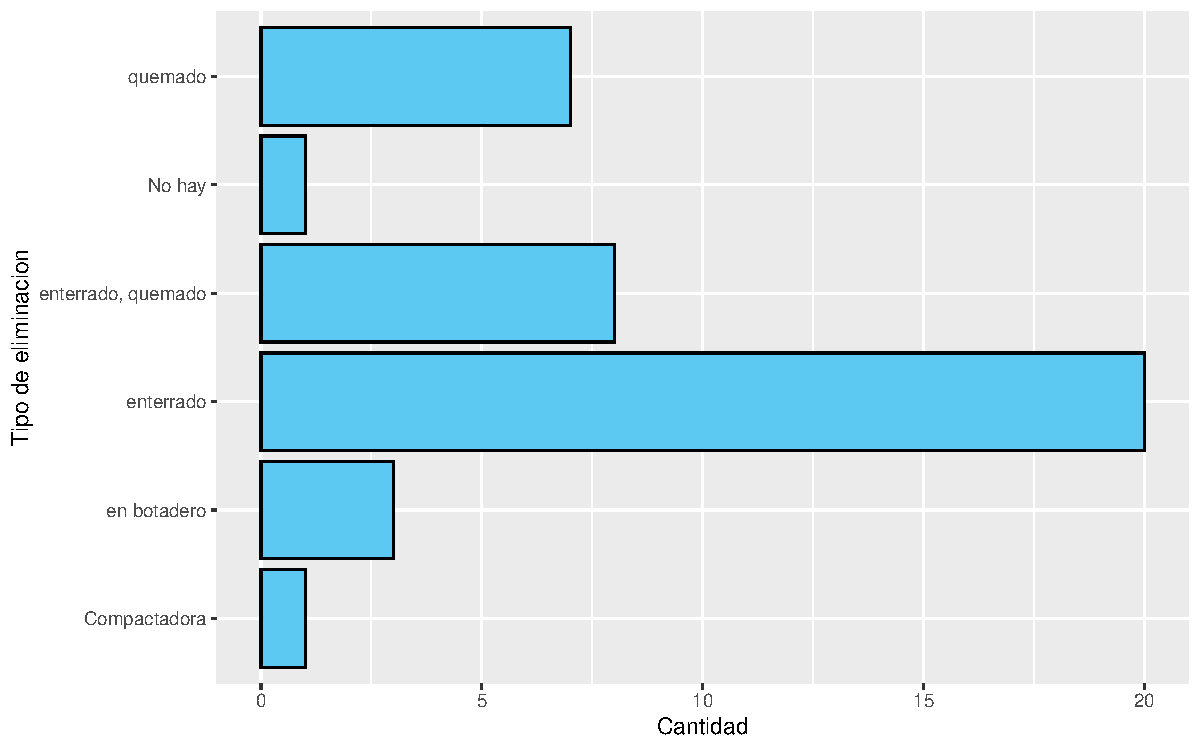
\includegraphics[width=\maxwidth]{figure/siete-1} 
\end{knitrout}
	\caption{Eliminacion de la basura en \comunidad}
	\end{figure}
	Los tipos de eliminacion con mayor frecuencia son enterrado y quemado, siendo el menor el uso de hoyo; se observa que el uso del recolector municipal es de los que tienen menos uso.\\
	\\
	Para la preparacion de sus alimentos las personas utilizan los siguientes combustibles:
	\begin{figure}[H]
	\centering
\begin{knitrout}
\definecolor{shadecolor}{rgb}{0.969, 0.969, 0.969}\color{fgcolor}
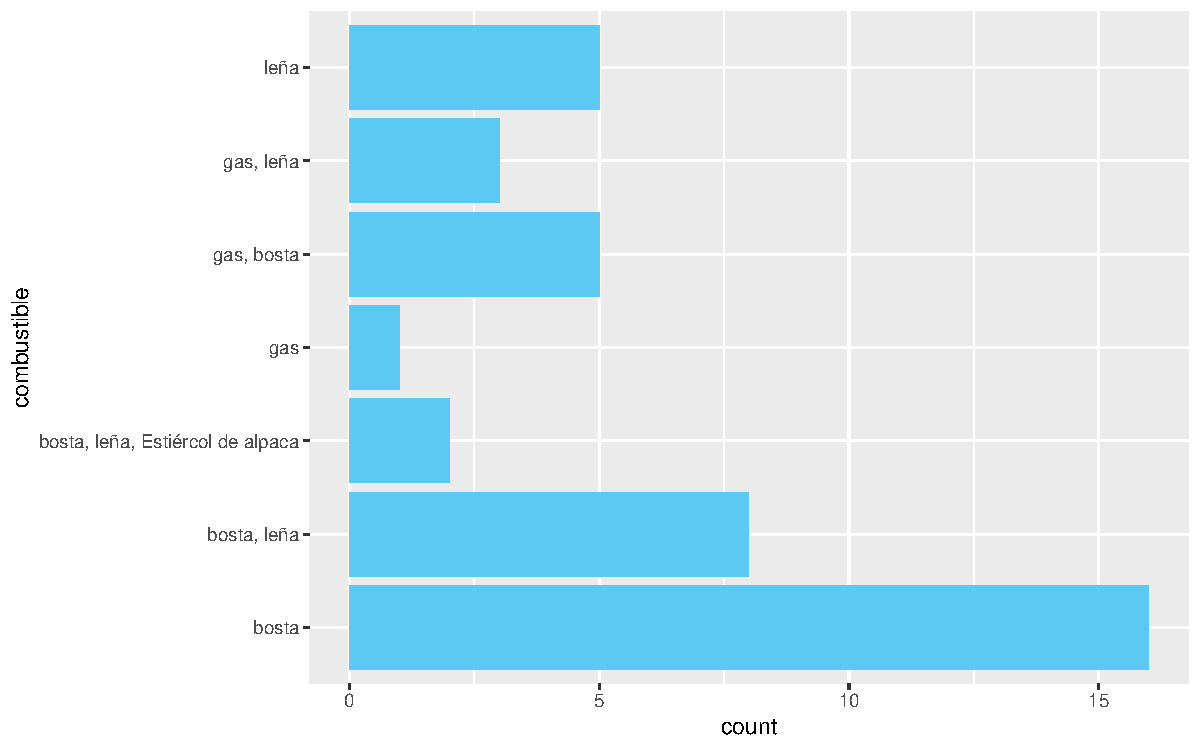
\includegraphics[width=\maxwidth]{figure/ocho-1} 
\end{knitrout}
	\caption{Uso de combustible para preparacion de alimentos en \comunidad}
	\end{figure}
	Los pobladores usan con mas frecuencia leña, luego gas, seguido de bosta y gas o gas leña; los pobladores indican que tienden a usar gas en las temporadas en las que no es posible obtener leña, se puede decudir que los pobladores tienen mayor preferencia por el uso de leña porque su uso es mas accesible y barato.\\
	\\
	Las enfermedades que mas aquejan a la poblacion son las siguientes:
	\begin{figure}[H]
	\centering
\begin{knitrout}
\definecolor{shadecolor}{rgb}{0.969, 0.969, 0.969}\color{fgcolor}
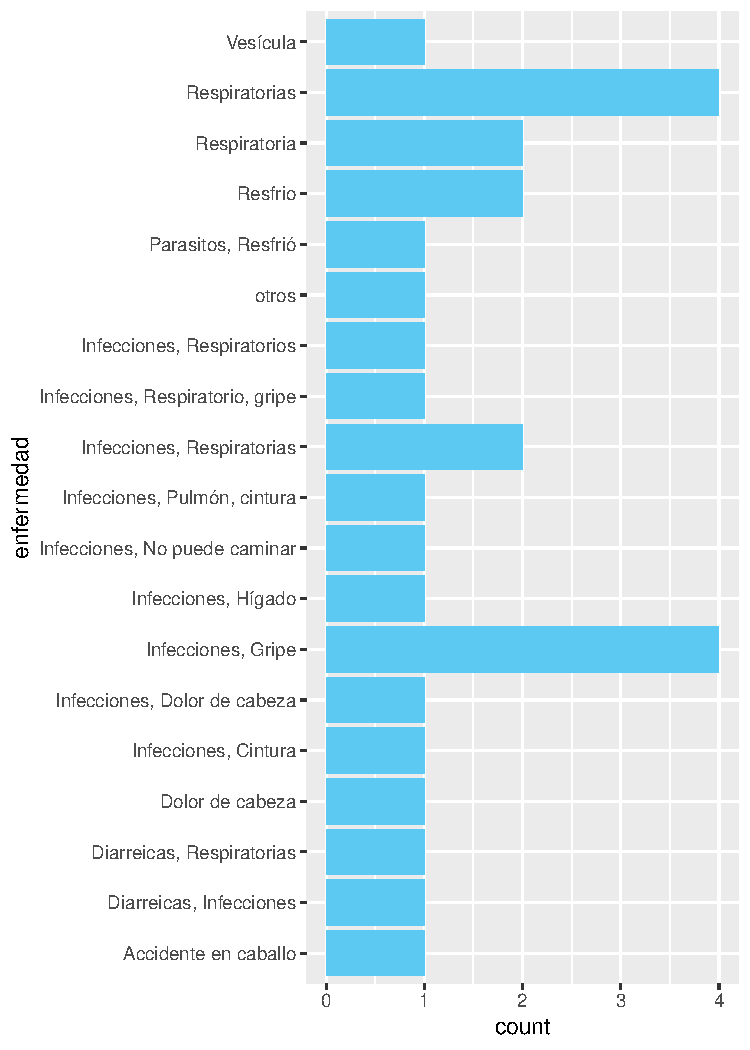
\includegraphics[width=\maxwidth]{figure/nueve-1} 
\end{knitrout}
	\caption{Enfermedades que aquejan a los pobladores de \comunidad}
	\end{figure}
	Se observa que las enfermedades diarreicas son las que mas aquejan a la poblacion, seguida de otras y ninguna.\\
	\\
	Las personas que sufren de alguna enfermedad se atienden en los siguientes:
	\begin{figure}[H]
	\centering
\begin{knitrout}
\definecolor{shadecolor}{rgb}{0.969, 0.969, 0.969}\color{fgcolor}
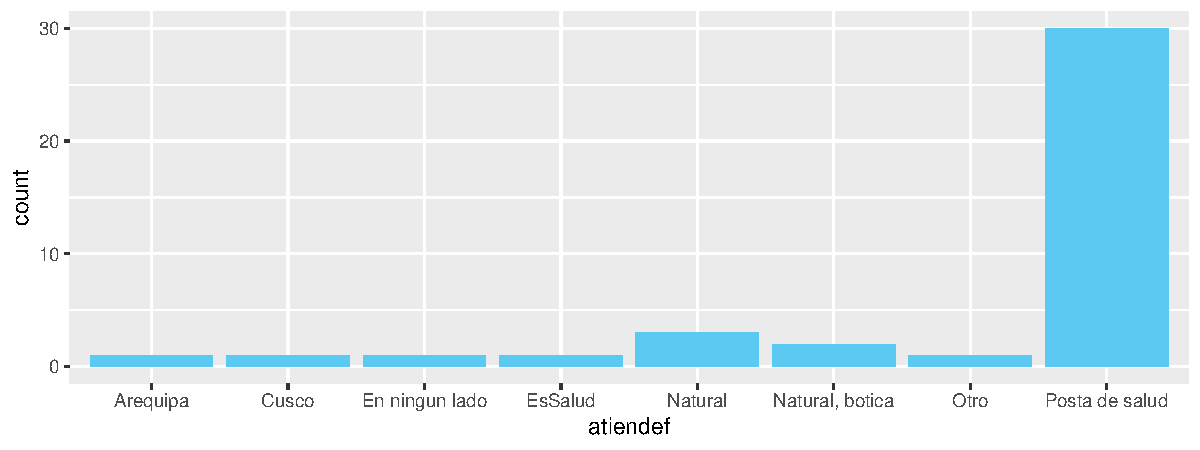
\includegraphics[width=\maxwidth]{figure/once-1} 
\end{knitrout}
	\caption{Lugar de atencion cuando se enferman}
	\end{figure}
  Como se puede observar la mayoria de los pobladores se atienden en la posta de salud mas cercana de su residencia.\\
  \\
	Se consulto si estas personas cuentan con seguro medico, de lo cual se obtuvo el siguiente resultado:
	\begin{figure}[H]
	\centering
\begin{knitrout}
\definecolor{shadecolor}{rgb}{0.969, 0.969, 0.969}\color{fgcolor}
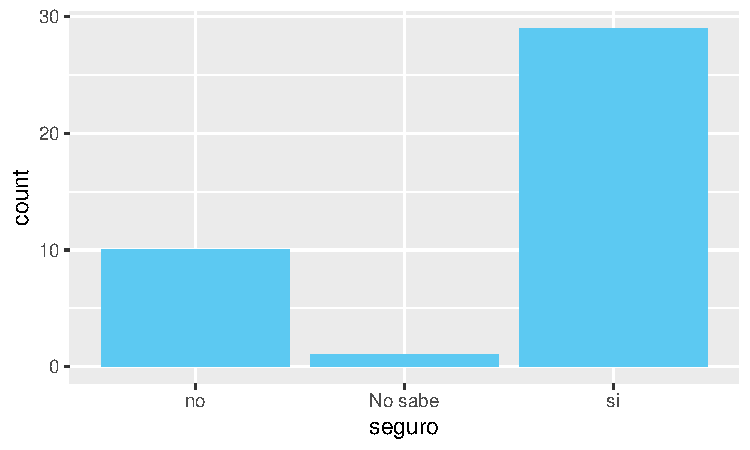
\includegraphics[width=\maxwidth]{figure/doce-1} 
\end{knitrout}
	\caption{Uso de un seguro medico}
	\end{figure}
	Se consulto respecto a la preferencia de emisoras radiales que se escucha, al respecto se tiene como primera emisora de preferencia la siguiente:
	\begin{figure}[H]
	\centering
\begin{knitrout}
\definecolor{shadecolor}{rgb}{0.969, 0.969, 0.969}\color{fgcolor}
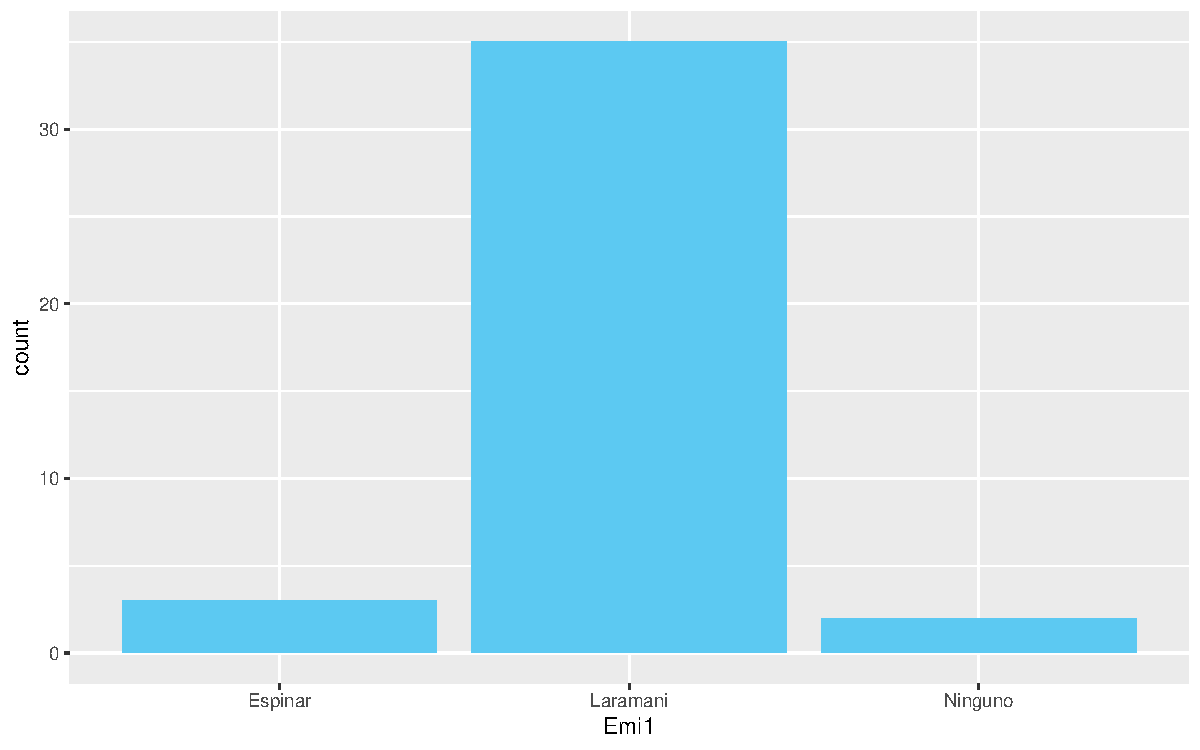
\includegraphics[width=\maxwidth]{figure/one-1} 
\end{knitrout}
	\caption{Primera emisora que se escucha}
	\end{figure}
	Como se puede observar la emisora con mayor audiencia es Laramani, seguido de emisora Espinar y las demas con menor porcentaje, como son Arequipa, Cadena Sur, Radio municipal, y San Luis.\\
	\\
	El horario que los encuestados prefieren escuchar es el siguiente:
	\begin{figure}[H]
	\centering
\begin{knitrout}
\definecolor{shadecolor}{rgb}{0.969, 0.969, 0.969}\color{fgcolor}
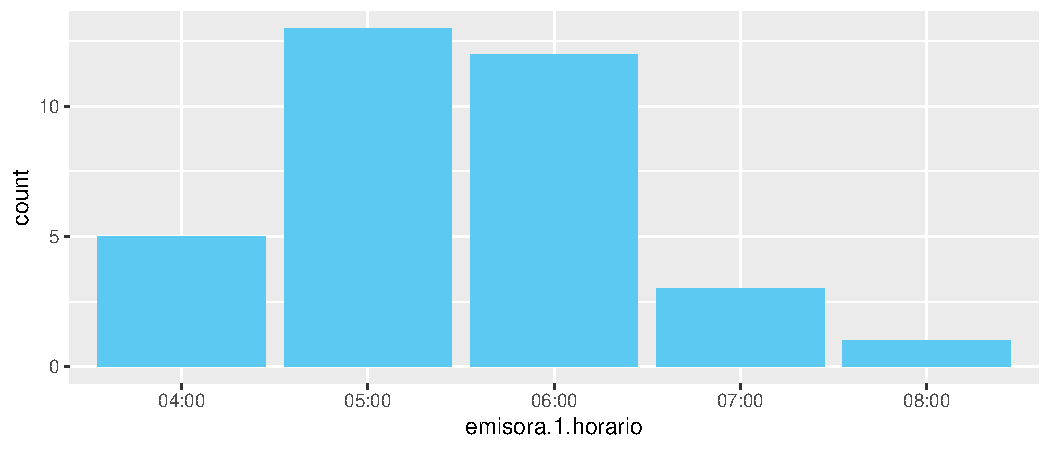
\includegraphics[width=\maxwidth]{figure/two-1} 
\end{knitrout}
	\caption{Horario de emisora preferida}
	\end{figure}
	
	\begin{figure}[H]
	\centering
\begin{knitrout}
\definecolor{shadecolor}{rgb}{0.969, 0.969, 0.969}\color{fgcolor}
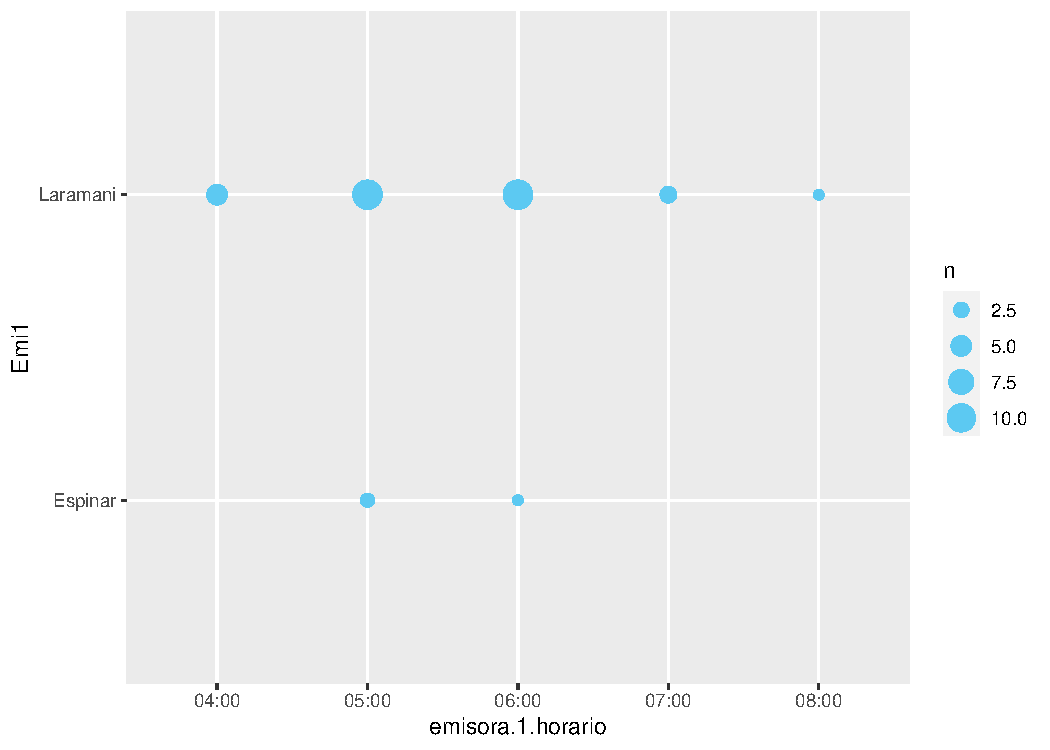
\includegraphics[width=\maxwidth]{figure/three-1} 
\end{knitrout}
	\caption{Emisoras y horarios preferidos}
	\end{figure}
	Como se puede observar todas las emisoras son sintonizadas a las 07:00 horas. Las emisoras que mas se escuchan en ese horario son Laramani y Espinar\\
	\\
	
	Se consulto respecto a la preferencia de emisoras radiales que se escucha, al respecto se tiene como primera emisora de preferencia la siguiente:
	\begin{figure}[H]
	\centering
\begin{knitrout}
\definecolor{shadecolor}{rgb}{0.969, 0.969, 0.969}\color{fgcolor}
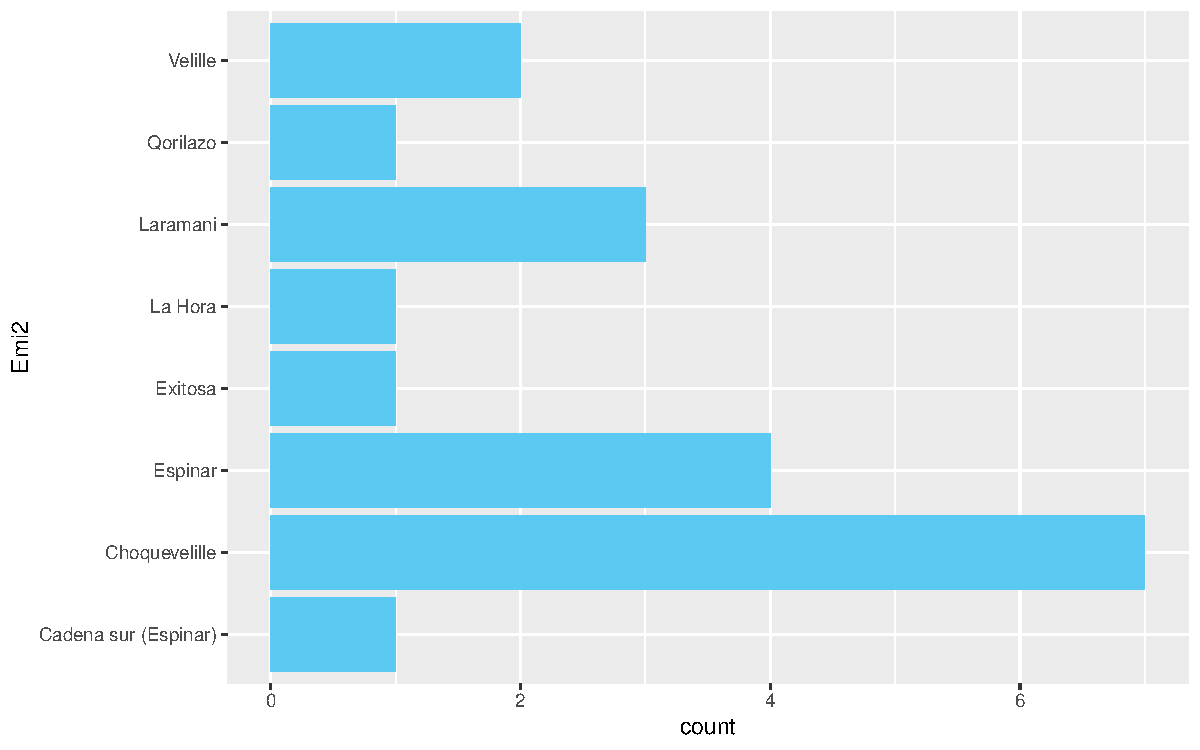
\includegraphics[width=\maxwidth]{figure/four-1} 
\end{knitrout}
	\caption{Seguna emisora que se escucha}
	\end{figure}
	De la segunda emisora que mas se escucha se identifico que tambien son Espinar y Laramani.\\
	\\
	El horario que los encuestados prefieren escuchar es el siguiente:
	\begin{figure}[H]
	\centering
\begin{knitrout}
\definecolor{shadecolor}{rgb}{0.969, 0.969, 0.969}\color{fgcolor}
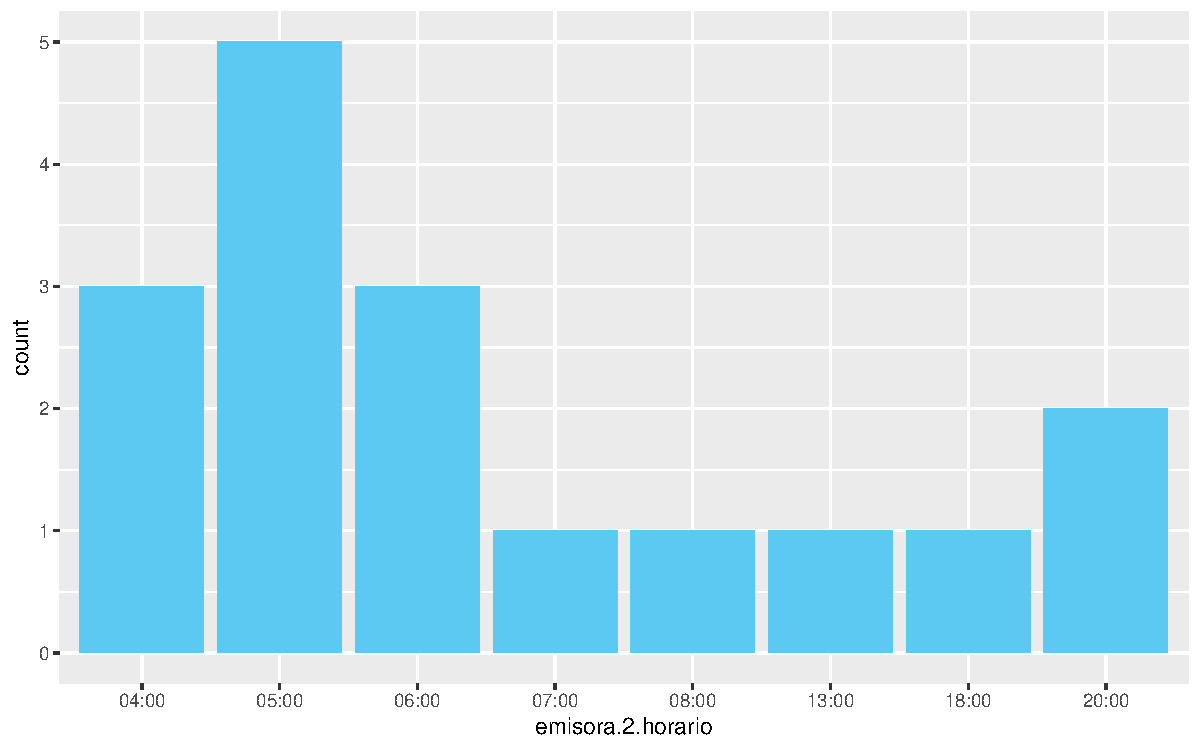
\includegraphics[width=\maxwidth]{figure/five-1} 
\end{knitrout}
	\caption{Horario de emisora preferida}
	\end{figure}
	
	\begin{figure}[H]
	\centering
\begin{knitrout}
\definecolor{shadecolor}{rgb}{0.969, 0.969, 0.969}\color{fgcolor}
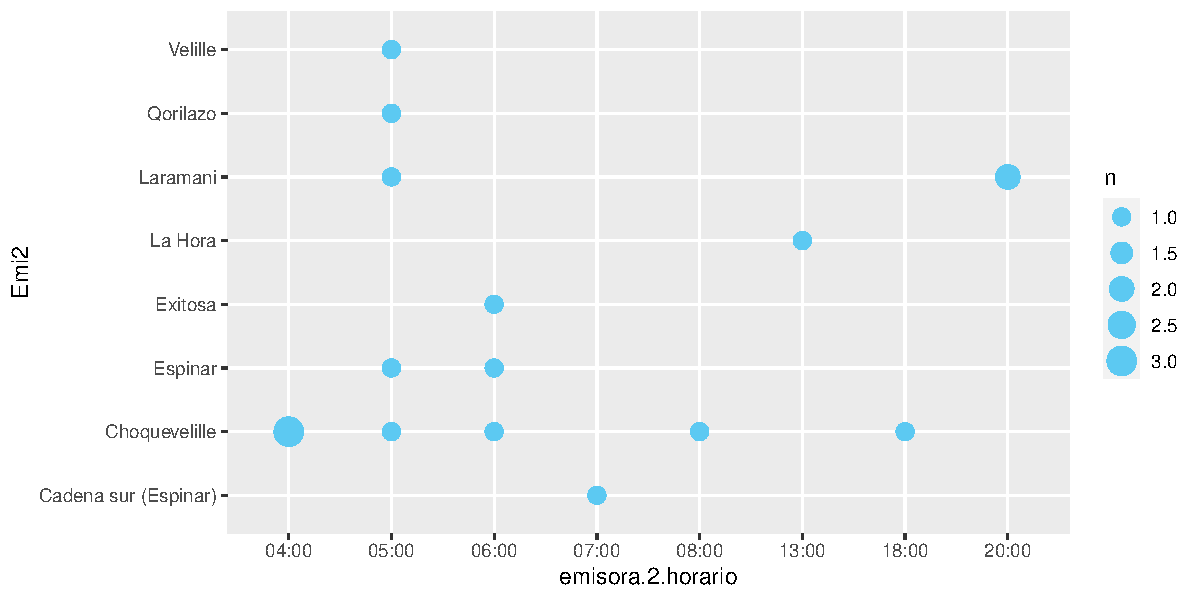
\includegraphics[width=\maxwidth]{figure/six-1} 
\end{knitrout}
	\caption{Emisoras y horarios preferidos}
	\end{figure}
	Se observa que aca tambien el horario preferido para escuchar la segunda emisora es a las 19:00 horas
	
	
	\section{Datos agropecuarios}
	De la actividad agropecuaria, se pregunto que cultivos como primera opcion realizan, de lo cual se obtuvo la siguiente informacion:
	\begin{figure}[H]
	\centering
\begin{knitrout}
\definecolor{shadecolor}{rgb}{0.969, 0.969, 0.969}\color{fgcolor}
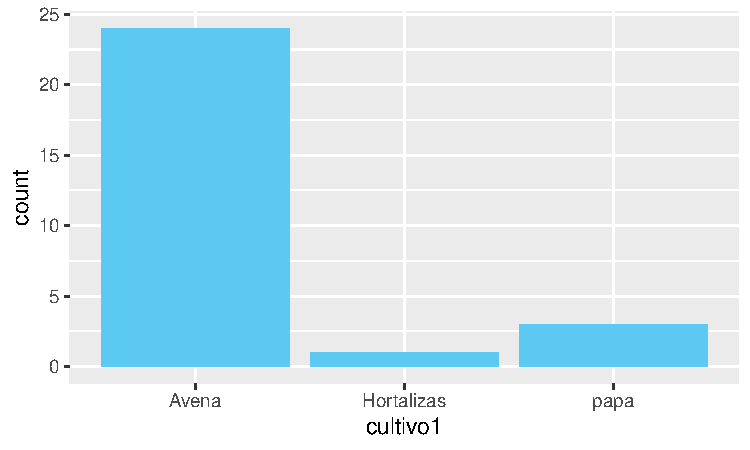
\includegraphics[width=\maxwidth]{figure/seven-1} 
\end{knitrout}
	\caption{Cultivo al que se dedican las personas}
	\end{figure}
	Se observa que el cultivo que a la que las personas se dedican en mayor proporcion es avena, seguido de papa y trebol.\\
	\\
	De la cantidad de cultivo se tiene lo siguiente:
	\begin{figure}[H]
	\centering
\begin{knitrout}
\definecolor{shadecolor}{rgb}{0.969, 0.969, 0.969}\color{fgcolor}\begin{kframe}


{\ttfamily\noindent\color{warningcolor}{\#\# Warning: NAs introducidos por coerción}}\end{kframe}
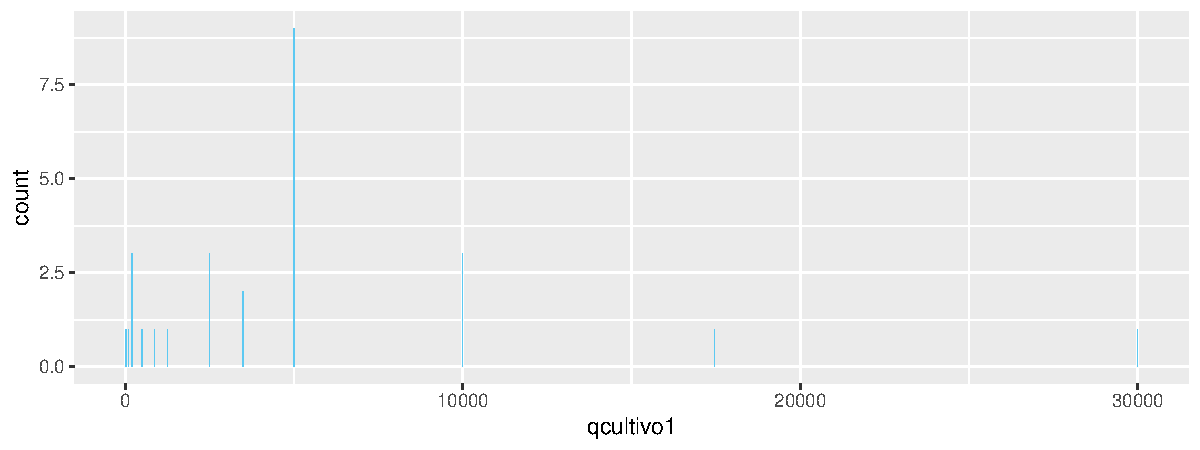
\includegraphics[width=\maxwidth]{figure/eight-1} 
\end{knitrout}
	\caption{Primera opcion de cultivo en \comunidad \- en cantidades}
	\end{figure}
	
	Se observa que el cultivo que mas se realiza es la avena del cual se tiene la cantidad de cultivo que mas se practica es en 5000.
	\begin{figure}[H]
	\centering
\begin{knitrout}
\definecolor{shadecolor}{rgb}{0.969, 0.969, 0.969}\color{fgcolor}\begin{kframe}


{\ttfamily\noindent\color{warningcolor}{\#\# Warning: NAs introducidos por coerción}}\end{kframe}
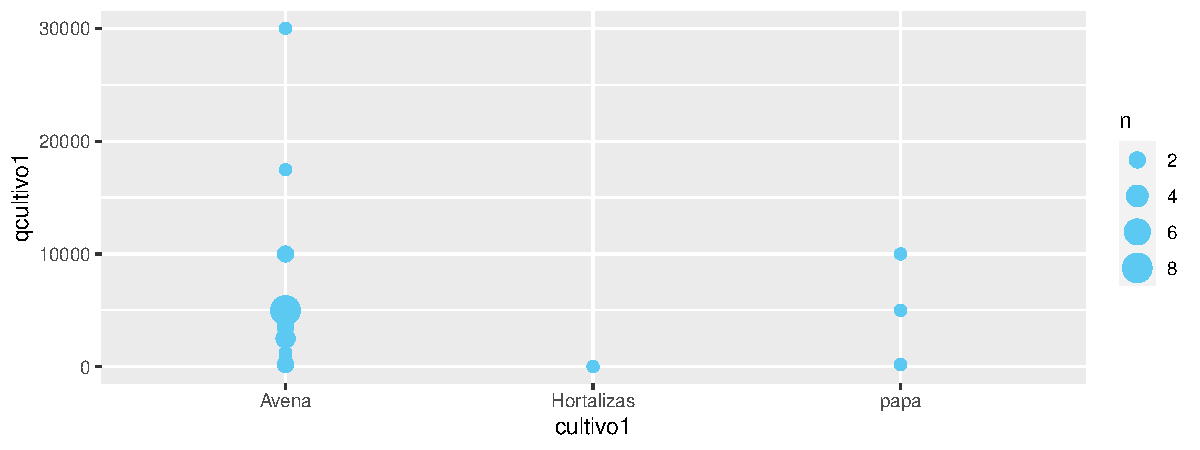
\includegraphics[width=\maxwidth]{figure/oneh-1} 
\end{knitrout}
	\caption{Cantidad de cultivo por producto}
	\end{figure}
	
	\begin{figure}[H]
	\centering
\begin{knitrout}
\definecolor{shadecolor}{rgb}{0.969, 0.969, 0.969}\color{fgcolor}
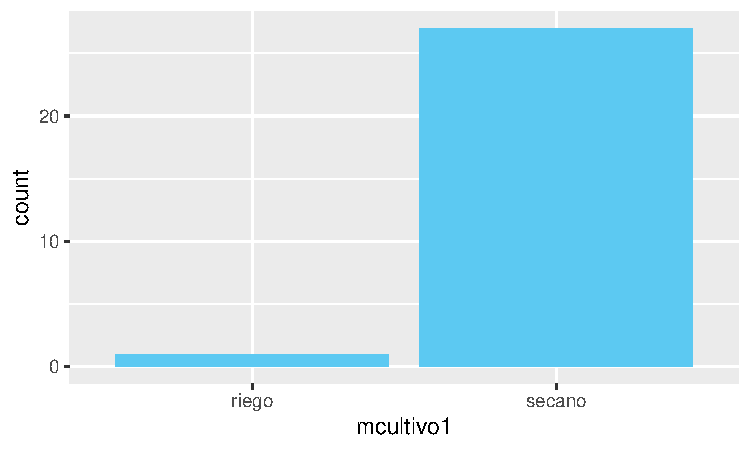
\includegraphics[width=\maxwidth]{figure/twelve-1} 
\end{knitrout}
	\caption{Metodo de cultivo de la primera opcion de cultivo}
	\end{figure}
	
	De la actividad agropecuaria, se pregunto que cultivos como segunda opcion realizan, de lo cual se obtuvo la siguiente informacion:
	\begin{figure}[H]
	\centering
\begin{knitrout}
\definecolor{shadecolor}{rgb}{0.969, 0.969, 0.969}\color{fgcolor}
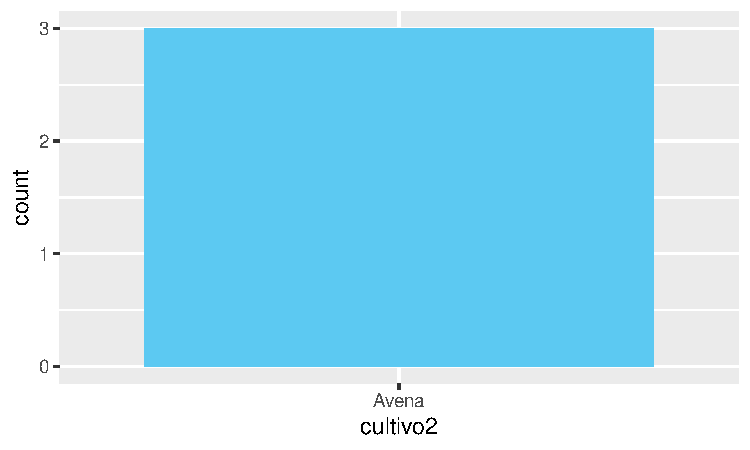
\includegraphics[width=\maxwidth]{figure/nine-1} 
\end{knitrout}
	\caption{Cultivo al que se dedican las personas como segunda opcion}
	\end{figure}
	Se observa que el cultivo que a la que las personas se dedican en mayor proporcion es avena, seguido de papa y trebol en la misma proporcion.\\
	\\
	De la cantidad de cultivo se tiene lo siguiente:
	\begin{figure}[H]
	\centering
\begin{knitrout}
\definecolor{shadecolor}{rgb}{0.969, 0.969, 0.969}\color{fgcolor}
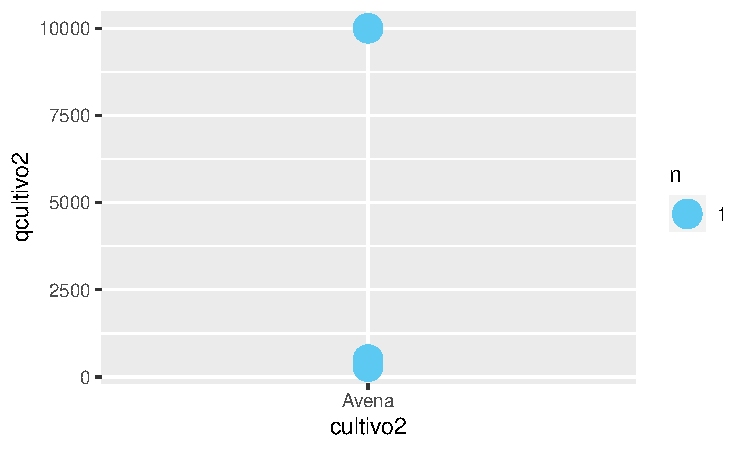
\includegraphics[width=\maxwidth]{figure/ten-1} 
\end{knitrout}
	\caption{Cantidad de cultivo de la segunda opcion de cultivo en \comunidad}
	\end{figure}
	Se observa que el cultivo que mas se realiza es la avena del cual se tiene la cantidad de cultivo que mas se practica es en 5000. Y en la cantidad de 500 se repite para evena y papa.
	\begin{figure}[H]
	\centering
\begin{knitrout}
\definecolor{shadecolor}{rgb}{0.969, 0.969, 0.969}\color{fgcolor}
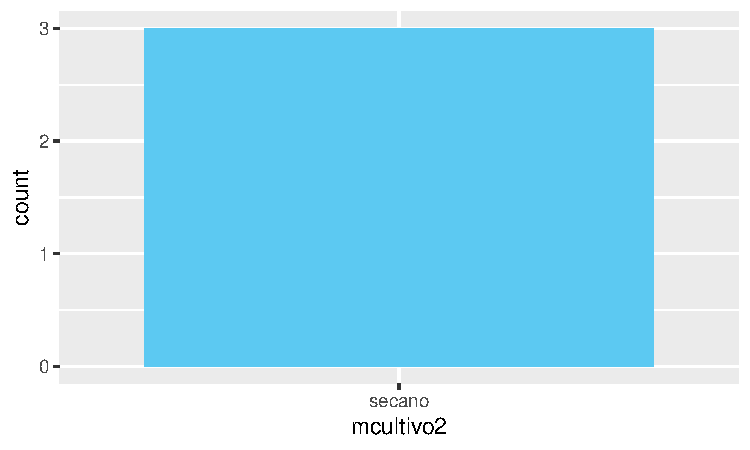
\includegraphics[width=\maxwidth]{figure/eleven-1} 
\end{knitrout}
	\caption{Metodo de cultivo de la segunda opcion de cultivo en \comunidad}
	\end{figure}
	
	
	De la actividad agropecuaria, se pregunto que animales cria segunda opcion, de lo cual se obtuvo la siguiente informacion:
	\begin{figure}[H]
	\centering
\begin{knitrout}
\definecolor{shadecolor}{rgb}{0.969, 0.969, 0.969}\color{fgcolor}\begin{kframe}
\begin{verbatim}
## 
##  Alpaca Alpacas    Vaca 
##      35       3       2
\end{verbatim}
\end{kframe}
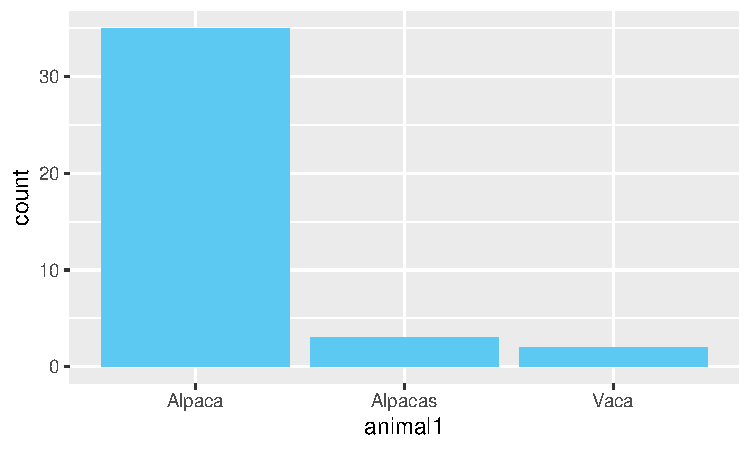
\includegraphics[width=\maxwidth]{figure/fifteen-1} 
\end{knitrout}
	\caption{Animales al que se dedican las personas como primera opcion}
	\end{figure}
	Se observa que la crianza a la que las personas se dedican en mayor proporcion es alpaca, seguida de ovejas en menor proporcion.\\
	\\
	De la cantidad de animales que crian se tiene lo siguiente:
	\begin{figure}[H]
	\centering
\begin{knitrout}
\definecolor{shadecolor}{rgb}{0.969, 0.969, 0.969}\color{fgcolor}
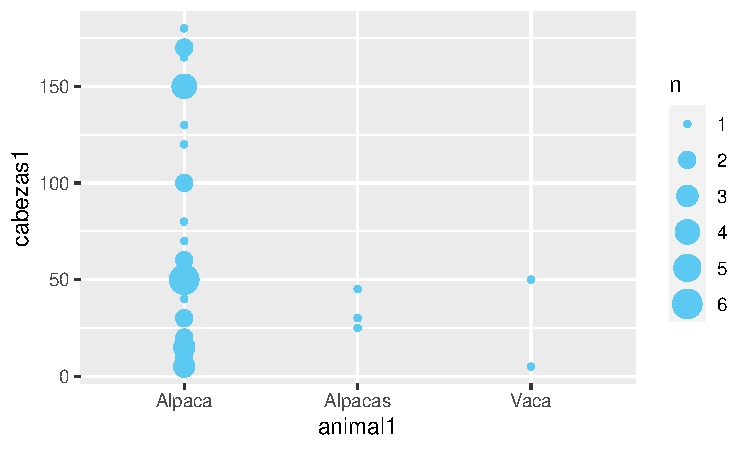
\includegraphics[width=\maxwidth]{figure/sixteen-1} 
\end{knitrout}
	\caption{Cantidad de animales criados de primera opcion en funcion a la cantidad y especie en \comunidad}
	\end{figure}
	
	\begin{figure}[H]
	\centering
\begin{knitrout}
\definecolor{shadecolor}{rgb}{0.969, 0.969, 0.969}\color{fgcolor}
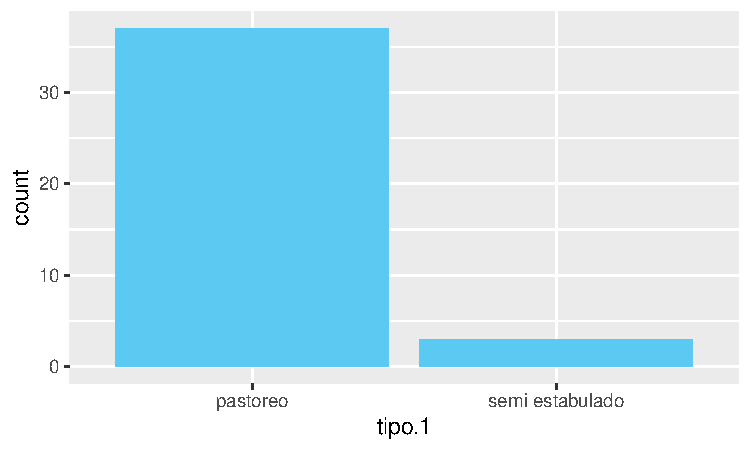
\includegraphics[width=\maxwidth]{figure/seventeen-1} 
\end{knitrout}
	\caption{Metodo de crianza de la primera opcion de crianza de animales en \comunidad}
	\end{figure}
	
	
	De la actividad agropecuaria, se pregunto que animales cria como segunda opcion, de lo cual se obtuvo la siguiente informacion:
	\begin{figure}[H]
	\centering
\begin{knitrout}
\definecolor{shadecolor}{rgb}{0.969, 0.969, 0.969}\color{fgcolor}
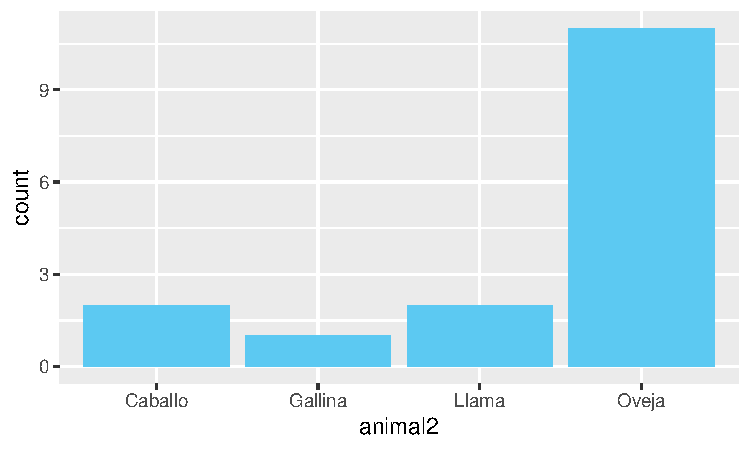
\includegraphics[width=\maxwidth]{figure/eighteen-1} 
\end{knitrout}
	\caption{Animales al que se dedican las personas como segunda opcion}
	\end{figure}
	Se observa que la crianza a la que las personas se dedican en mayor proporcion es oveja, seguida de llamas y alpaca en menor proporcion.\\
	\\
	De la cantidad de animales que crian se tiene lo siguiente:
	\begin{figure}[H]
	\centering
\begin{knitrout}
\definecolor{shadecolor}{rgb}{0.969, 0.969, 0.969}\color{fgcolor}
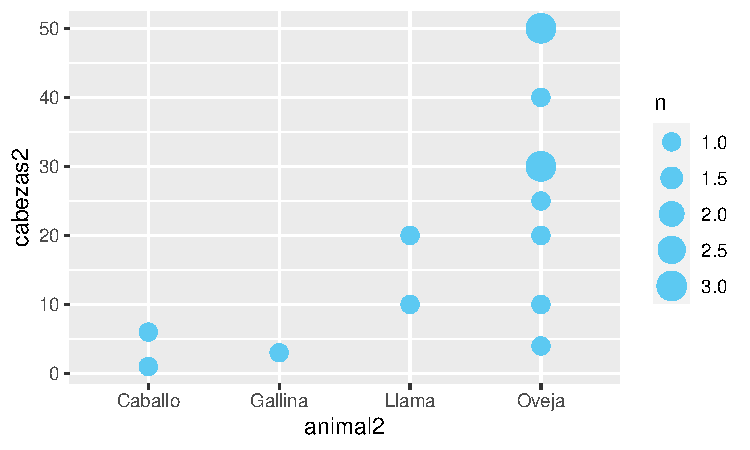
\includegraphics[width=\maxwidth]{figure/nineteen-1} 
\end{knitrout}
	\caption{Cantidad de animales criados de segunda opcion en funcion a la cantidad y especie en \comunidad}
	\end{figure}
	
	\begin{figure}[H]
	\centering
\begin{knitrout}
\definecolor{shadecolor}{rgb}{0.969, 0.969, 0.969}\color{fgcolor}
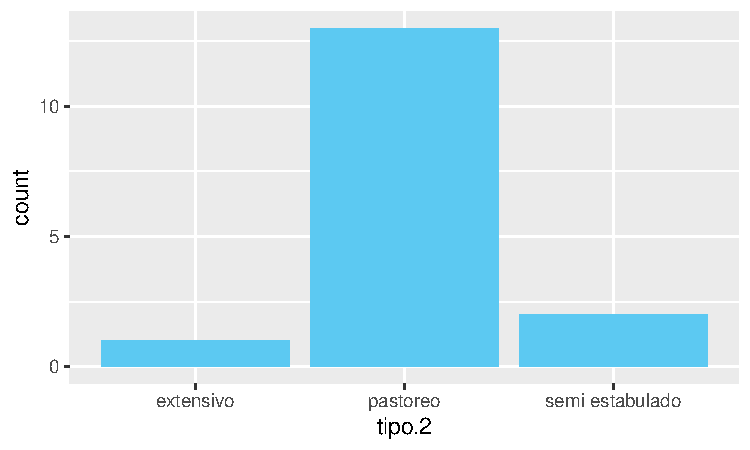
\includegraphics[width=\maxwidth]{figure/twenty-1} 
\end{knitrout}
	\caption{Metodo de crianza de la segunda opcion de crianza de animales en \comunidad}
	\end{figure}
	
	
	De la actividad agropecuaria, se pregunto que animales cria como tercera opcion, de lo cual se obtuvo la siguiente informacion:
	\begin{figure}[H]
	\centering
\begin{knitrout}
\definecolor{shadecolor}{rgb}{0.969, 0.969, 0.969}\color{fgcolor}
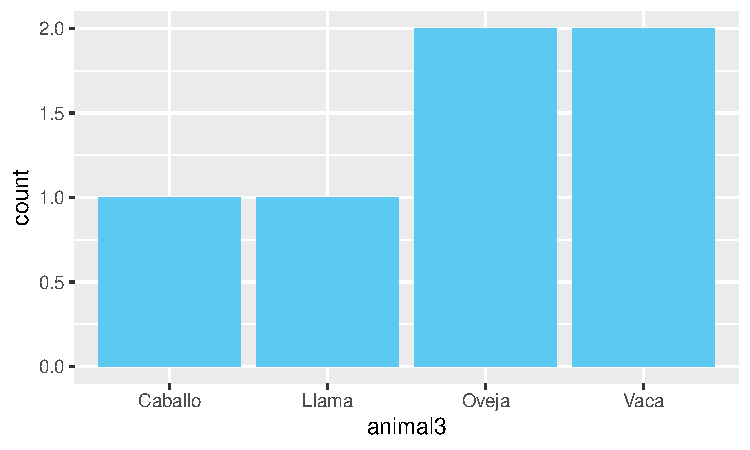
\includegraphics[width=\maxwidth]{figure/twenty_one-1} 
\end{knitrout}
	\caption{Animales al que se dedican las personas como tercera opcion}
	\end{figure}
	Se observa que la crianza a la que las personas se dedican en mayor proporcion es oveja, seguida de llamas y alpaca en menor proporcion.\\
	\\
	De la cantidad de animales que crian se tiene lo siguiente:
	\begin{figure}[H]
	\centering
\begin{knitrout}
\definecolor{shadecolor}{rgb}{0.969, 0.969, 0.969}\color{fgcolor}
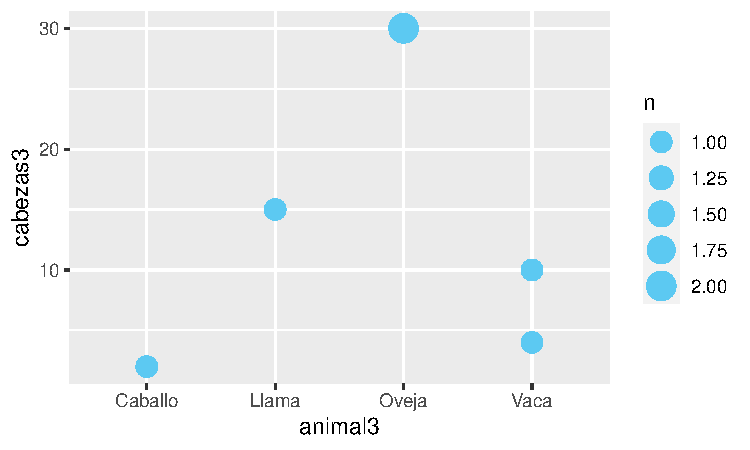
\includegraphics[width=\maxwidth]{figure/twenty_two-1} 
\end{knitrout}
	\caption{Cantidad de animales criados de tercera opcion en funcion a la cantidad y especie en \comunidad}
	\end{figure}
	Del metodo de crianza de esta opcion de animales se tiene lo siguiente:
	\begin{figure}[H]
	\centering
\begin{knitrout}
\definecolor{shadecolor}{rgb}{0.969, 0.969, 0.969}\color{fgcolor}
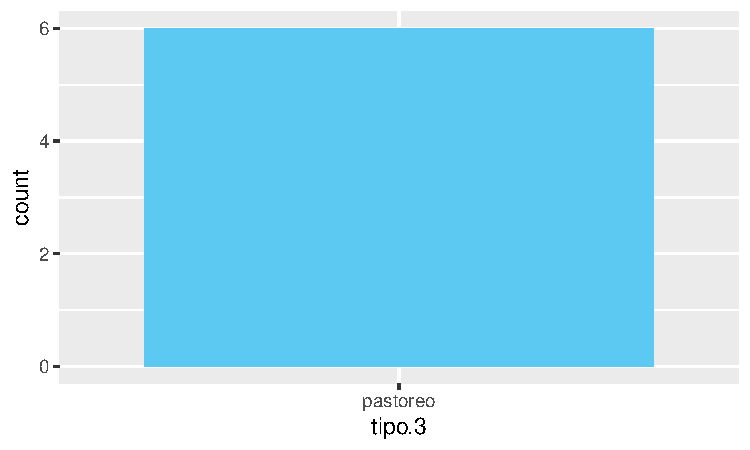
\includegraphics[width=\maxwidth]{figure/twenty_three-1} 
\end{knitrout}
	\caption{Metodo de crianza de la tercera opcion de crianza de animales en \comunidad}
	\end{figure}
	
	
	
	\section{Recurso hidrico}
	De las personas que acceden al servicio de las qochas se identifico que solo esta cantidad accede al servicio:
	\begin{figure}[H]
	\centering
\begin{knitrout}
\definecolor{shadecolor}{rgb}{0.969, 0.969, 0.969}\color{fgcolor}
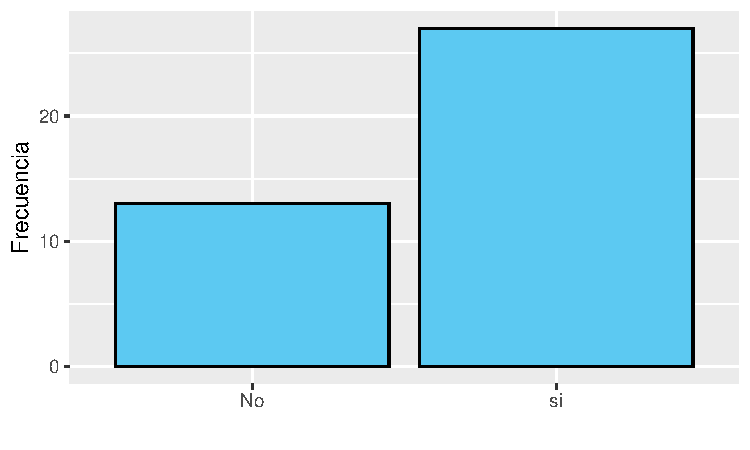
\includegraphics[width=\maxwidth]{figure/trece-1} 
\end{knitrout}
	\caption{Acceso al recurso}
	\end{figure}
	Se puede observar que la mayoria de los pobladores no acceden al recurso en menor medida si.\\
	\\
	De los propietarios de la qocha se identifico las siguientes respuestas:
	\begin{figure}[H]
	\centering
\begin{knitrout}
\definecolor{shadecolor}{rgb}{0.969, 0.969, 0.969}\color{fgcolor}
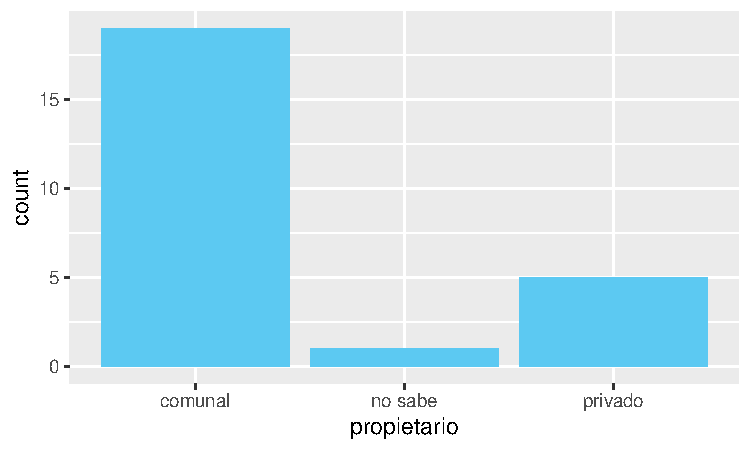
\includegraphics[width=\maxwidth]{figure/catorce-1} 
\end{knitrout}
	\caption{Propietario del recurso}
	\end{figure}
	Se identifica que la mayoria de los pobladores identifica a la comunidad como propietaria de las qochas en consulta, un porcentaje menor es de propiedad privada y uno muy bajo reconoce como propietario al estado.\\
	\\
	Del uso que se da se tiene lo siguiente:
	\begin{figure}[H]
	\centering
\begin{knitrout}
\definecolor{shadecolor}{rgb}{0.969, 0.969, 0.969}\color{fgcolor}
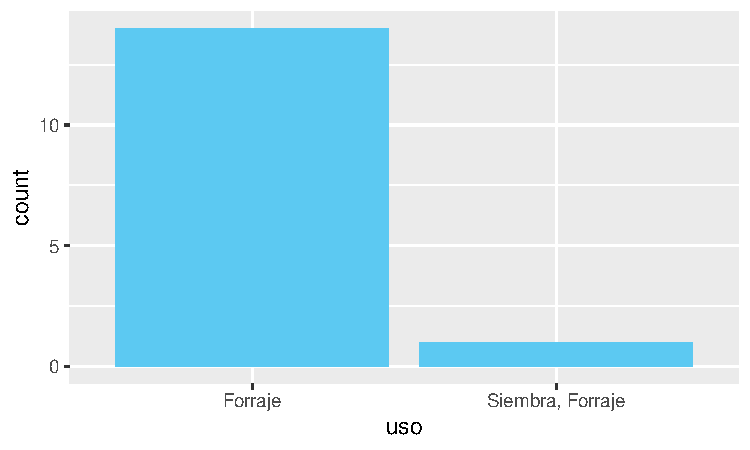
\includegraphics[width=\maxwidth]{figure/quince-1} 
\end{knitrout}
	\caption{Uso del recurso}
	\end{figure}
	De los pobladores que tienen acceso al uso del recursos, se identifico que todos lo utilizan para forraje y una parte utiliza para siembra y forraje.\\
	\\
	Se consulto si los beneficiarios estan satisfechos con el servicio de las qochas y se tuvo como resultado lo siguiente:
	\begin{figure}[H]
	\centering
\begin{knitrout}
\definecolor{shadecolor}{rgb}{0.969, 0.969, 0.969}\color{fgcolor}
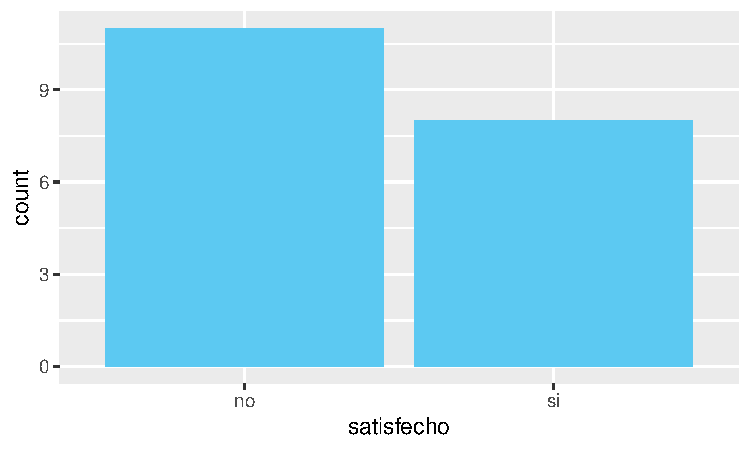
\includegraphics[width=\maxwidth]{figure/dieciseis-1} 
\end{knitrout}
	\caption{Satisfaccion con el uso del recurso}
	\end{figure}
	Como se puede observar es mayor la poblacion que esta insatisfecha con el uso del recurso, se concluye que este no cuenta con un nivel adecuado para brindar el servicio.\\
	\\
	Se consulto que otra fuente de agua usa en reemplazo del recurso, de los cual se tiene como resultado:
	\begin{figure}[H]
	\centering
\begin{knitrout}
\definecolor{shadecolor}{rgb}{0.969, 0.969, 0.969}\color{fgcolor}
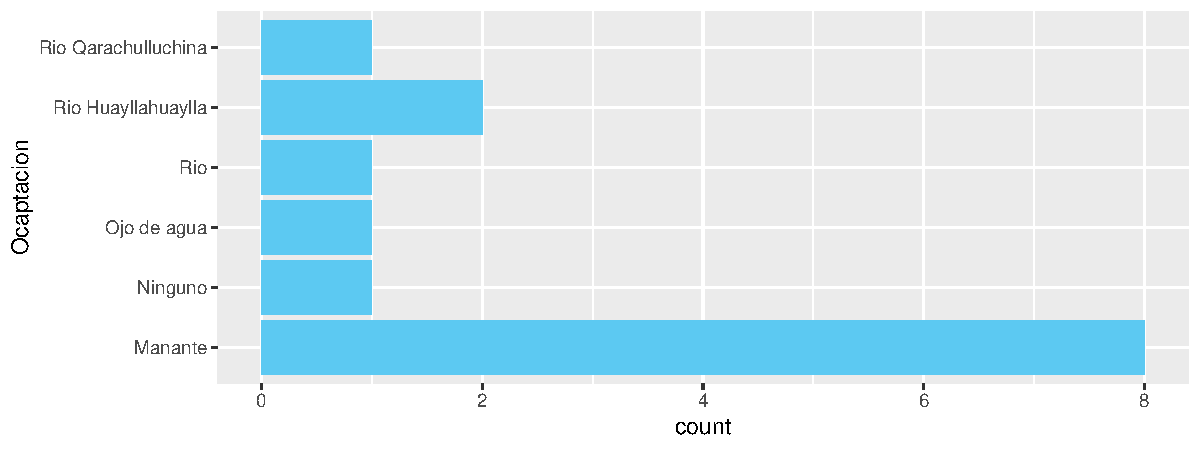
\includegraphics[width=\maxwidth]{figure/diecisiete-1} 
\end{knitrout}
	\caption{Otro recurso que suple la oferta del recurso}
	\end{figure}
	Se observa que los recursos que reemplazan son embalse y manantial, siendo el segundo el de mayor uso.\\
	\\
	Se consulto cual es la razon por la que los usuarios no se sienten satisfechos y se identifico lo siguiente:
	\begin{figure}[H]
	\centering
\begin{knitrout}
\definecolor{shadecolor}{rgb}{0.969, 0.969, 0.969}\color{fgcolor}
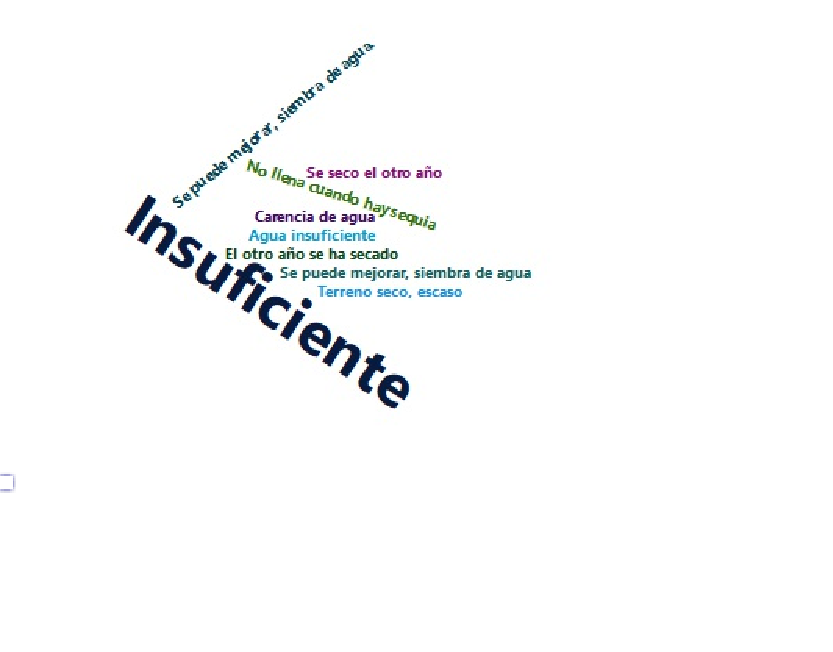
\includegraphics[width=\maxwidth]{figure/dieciocho-1} 
\end{knitrout}
	\caption{Razon de descontento}
	\end{figure}
	Debido a que las respuestas no son alternativas y son abiertas, se opto por utilizar mineria de datos para estas, de la cual se ha identificado que la opinion con mayor frecuencia es que el descontento se debe a la poca disponibilidad de agua.
	\section{Aspectos socioeconomicos}
	Se consulto cuantos integrantes de su familia trabajan, de lo cual se tiene la siguiente informacion
	\begin{figure}[H]
	\centering
\begin{knitrout}
\definecolor{shadecolor}{rgb}{0.969, 0.969, 0.969}\color{fgcolor}
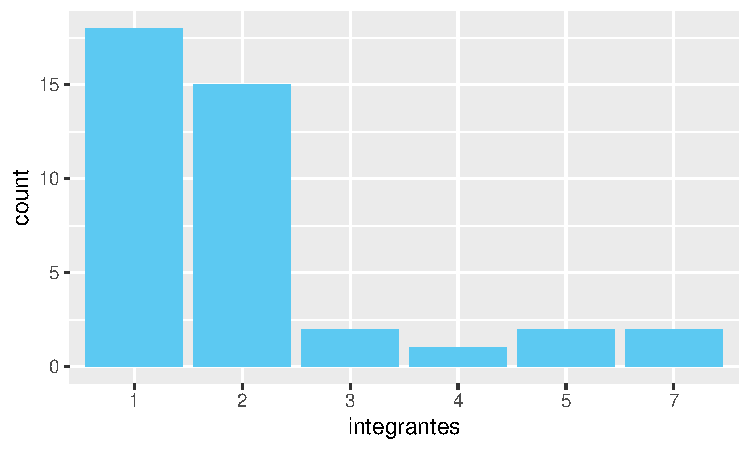
\includegraphics[width=\maxwidth]{figure/diecinueve-1} 
\end{knitrout}
	\caption{cantidad de integrantes que trabajan en la familia}
	\end{figure}
	Se observa que en la mayoria de familias quienes trabajan son dos integrantes, seguido de tres.\\
	\\
  Se consulto el ingreso familiar promedio de la familia de lo cual se tiene lo siguiente:
	\begin{figure}[H]
	\centering
\begin{knitrout}
\definecolor{shadecolor}{rgb}{0.969, 0.969, 0.969}\color{fgcolor}\begin{kframe}


{\ttfamily\noindent\color{warningcolor}{\#\# Warning: NAs introducidos por coerción}}\end{kframe}
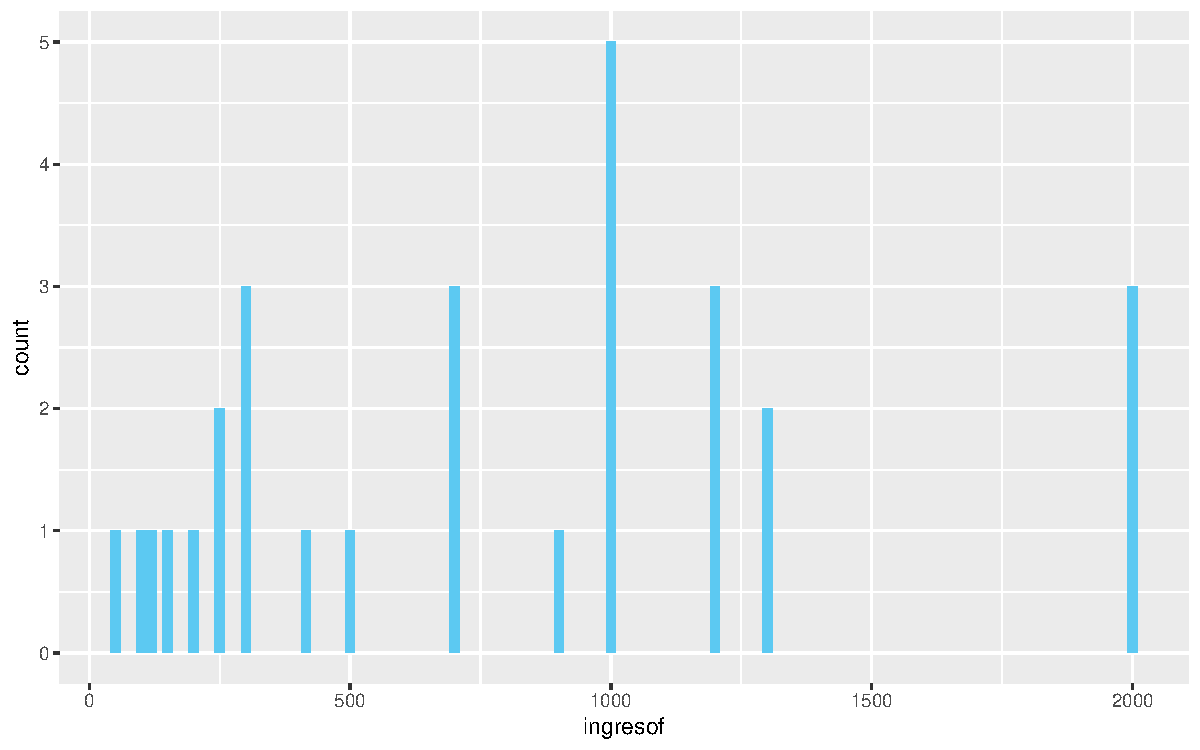
\includegraphics[width=\maxwidth]{figure/veinte-1} 
\end{knitrout}
	\caption{Ingreso promedio de las familias de \comunidad}
	\end{figure}
	Se puede observar que las familias tienen como ingreso mensual en promedio 1000\\
	\\
	Combinando la cantidad de integrantes que trabajan y el ingreso promedio mensual, se tiene lo siguiente:
	
	\begin{figure}[H]
	\centering
\begin{knitrout}
\definecolor{shadecolor}{rgb}{0.969, 0.969, 0.969}\color{fgcolor}\begin{kframe}


{\ttfamily\noindent\color{warningcolor}{\#\# Warning: NAs introducidos por coerción}}

{\ttfamily\noindent\color{warningcolor}{\#\# Warning: Removed 11 rows containing non-finite values (`stat\_sum()`).}}\end{kframe}
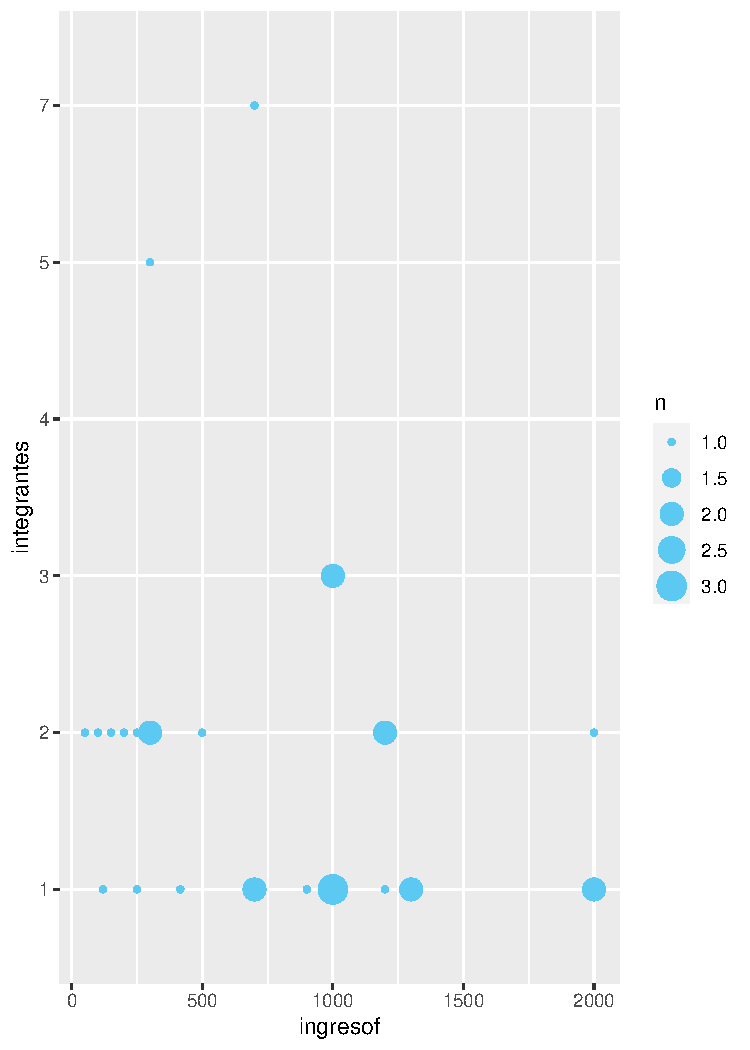
\includegraphics[width=\maxwidth]{figure/nose-1} 
\end{knitrout}
	\caption{Ingreso promedio de las familias de \comunidad en funciona a la cantidad de persionas que trabajan}
	\end{figure}

	\section{Aspectos sociales y culturales}
	De la religion que los encuestados creen se tiene la siguiente informacion:
	\begin{figure}[H]
	\centering
\begin{knitrout}
\definecolor{shadecolor}{rgb}{0.969, 0.969, 0.969}\color{fgcolor}
\includegraphics[width=\maxwidth]{figure/veintiuno-1} 
\end{knitrout}
	\caption{Religion de los pobladores de \comunidad}
	\end{figure}
	Se puede observar que la mayoria de los encuestados es de religion catolica y otras, en menor proporcion, seguido de Cristiano.\\
	\\
	De la pregunta respecto a si alguna organizacion cultural se dedica a la realizacion de las actividades de las qochas
	\begin{figure}[H]
	\centering
\begin{knitrout}
\definecolor{shadecolor}{rgb}{0.969, 0.969, 0.969}\color{fgcolor}
\includegraphics[width=\maxwidth]{figure/veintidos-1} 
\end{knitrout}
	\caption{Organizacion dedicada a actividades culturales en la qocha}
	\end{figure}
	Se observa que la mayoria de los pobladores indica que no existe alguna organizacion dedicada a la realizacion de actividades culturales en la qocha, mientras que solo una persona indica que si.  
	\section{Aspectos de gestion}
	De la consulta de la existencia de algun comite encargardo del funcionamiento de la qocha se obtuvo lo siguiente:
	\begin{figure}[H]
	\centering
\begin{knitrout}
\definecolor{shadecolor}{rgb}{0.969, 0.969, 0.969}\color{fgcolor}
\includegraphics[width=\maxwidth]{figure/veintitres-1} 
\end{knitrout}
	\caption{Comite encargado de la gestion del uso de la qocha en \comunidad}
	\end{figure}
	Se observa que la mayoria de los encuestados indican que no existe un comite de gestion encargado del uso de la qocha.\\
	\\
	Existe alguna organizacion externa dedicada al cuidado de la qocha, de la cual se tiene la siguiente respuesta
	\begin{figure}[H]
	\centering
\begin{knitrout}
\definecolor{shadecolor}{rgb}{0.969, 0.969, 0.969}\color{fgcolor}
\includegraphics[width=\maxwidth]{figure/veintiseis-1} 
\end{knitrout}
	\caption{Organizacion externa encargada del cuidado de la qocha}
	\end{figure}
	Se observa que todos los encuestados indican que no existe una organizacion externa encargada del cuidado de qochas en \comunidad.\\
	\\
	Se explico informacion respecto a los beneficios del proyecto, por lo que se consulto si la persona estaria dispuesta en apoyar durante la fase de funcionamiento que comprende la operacion y mantenimiento, de lo cual se tiene la siguiente respuesta:
	\begin{figure}[H]
	\centering
\begin{knitrout}
\definecolor{shadecolor}{rgb}{0.969, 0.969, 0.969}\color{fgcolor}
\includegraphics[width=\maxwidth]{figure/veintisiete-1} 
\end{knitrout}
	\caption{Disposicion de apoyo durante la ejecucion del proyecto}
	\end{figure}
	Se observa que la mayoria de los encuestados estarian dispuestos a apoyar durante la fase de ejecucion del proyecto.\\
	\\
	Explicada la constitucion de un comite encargado de la etapa de funcionamiento del proyecto se consulto la predisposicion de los encuestados a pagar una cuata maxima, de la cual se obtuvo las siguientes cantidades:
	\begin{figure}[H]
	\centering
\begin{knitrout}
\definecolor{shadecolor}{rgb}{0.969, 0.969, 0.969}\color{fgcolor}
\includegraphics[width=\maxwidth]{figure/veintiocho-1} 
\end{knitrout}
	\caption{Disposicion a pagar cuota durante el periodo de funcionamiento del proyecto}
	\end{figure}
	Se puede observar que entre quienes esten dispuestos a pagar y no, la proporcion es muy cercana, siendo mas alta quienes si apoyarian, solo por una persona.\\
	\\
	De la consulta respecto a la percepcion de un adecuado uso de las qochas por parte de las personas, se tiene la siguiente informacion:
	\begin{figure}[H]
	\centering
\begin{knitrout}
\definecolor{shadecolor}{rgb}{0.969, 0.969, 0.969}\color{fgcolor}
\includegraphics[width=\maxwidth]{figure/veintinueve-1} 
\end{knitrout}
	\caption{Percepcion de uso adecuado de las qochas}
	En este caso las dos alternativas son muy cercanas en proporcion, ganando por un reducido margen un uso adecuado.
	\end{figure}
	En este caso 
	\section{Aspectos de medio ambiente}
	Perjuicio en la actividad agropecuaria debido al cambio climatico
	\begin{figure}[H]
	\centering
\begin{knitrout}
\definecolor{shadecolor}{rgb}{0.969, 0.969, 0.969}\color{fgcolor}
\includegraphics[width=\maxwidth]{figure/treinta-1} 
\end{knitrout}
	\caption{Perjuicio en la actividad agropecuaria debido al cambio climatico}
	\end{figure}
	Como se aprecia los perjuicios producidos por el cambio climatico identificados por los encuestados son los siguientes: no hay nevados, poca agua, friaje y menor produccion.\\
	\\
	Especies de flora identificadas en la qocha
	
	\begin{figure}[H]
	\centering
\begin{knitrout}
\definecolor{shadecolor}{rgb}{0.969, 0.969, 0.969}\color{fgcolor}
\includegraphics[width=\maxwidth]{figure/treintayuno-1} 
\end{knitrout}
	\caption{Especies de flora identificadas en la qocha}
	\end{figure}
	Se puede observar que las especies de flora identificadas es Ch'inki y Pasto, mientras que las demas son Ichu, Totora y Ajuya.\\
	\\
	Especies de fauna identificadas en la qocha
	\begin{figure}[H]
	
	\centering
\begin{knitrout}
\definecolor{shadecolor}{rgb}{0.969, 0.969, 0.969}\color{fgcolor}
\includegraphics[width=\maxwidth]{figure/treintaydos-1} 
\end{knitrout}
	\caption{Especies de fauna identificadas en la qocha}
	\end{figure}
	Se observa que la especie de fauna identificada coon mayor frecuencia es Pato, seguido de Huallata y Parihuanas.\\
	\\
	Especies vegetales nativas en extincion.
	\begin{figure}[H]
	\centering
\begin{knitrout}
\definecolor{shadecolor}{rgb}{0.969, 0.969, 0.969}\color{fgcolor}
\includegraphics[width=\maxwidth]{figure/treintaytres-1} 
\end{knitrout}
	\caption{Especies vegetales en extincion}
	\end{figure}
	De las especies vegetales en peligrro de extincion, se ha identificado a la Yareta, Q'oya y Chinki.\\
	\\
	Modificaciones identificadas en la turba de la qocha.
	\begin{figure}[H]
	\centering
\begin{knitrout}
\definecolor{shadecolor}{rgb}{0.969, 0.969, 0.969}\color{fgcolor}
\includegraphics[width=\maxwidth]{figure/treintaycuatro-1} 
\end{knitrout}
	\caption{Alteraciones de la turba en la qocha}
	\end{figure}
	Se observa que los pobladores identifican que la turba se esta secando y desapareciendo.\\
	\\
	Alteraciones en la precipitacion pluvial en la zona de la qocha
	\begin{figure}[H]
	\centering
\begin{knitrout}
\definecolor{shadecolor}{rgb}{0.969, 0.969, 0.969}\color{fgcolor}
\includegraphics[width=\maxwidth]{figure/treintaycinco-1} 
\end{knitrout}
	\caption{Alteraciones pluviales en las zonas de qochas}
	\end{figure}
	La mayor alteracion pluvial que se ha indetificado es que hay menos lluvias en la zona de las qochas. \\
	\\
	Alteraciones en el suelo en la zona de la qocha
		\begin{figure}[H]
	\centering
\begin{knitrout}
\definecolor{shadecolor}{rgb}{0.969, 0.969, 0.969}\color{fgcolor}
\includegraphics[width=\maxwidth]{figure/treintayseis-1} 
\end{knitrout}
	\caption{Alteraciones en el suelo de las zonas de qochas}
	\end{figure}
	
	\begin{center}
		\textbf{Atentamente}
	\end{center}
	
	
	\begin{figure}[H]
		\centering
		\includegraphics[scale=0.35]{H:/Gore Cusco/img/firma}
	\end{figure}
	\thispagestyle{lastpage}




\end{document}
